\chapter{Mapeos conformes} \label{chap:background}
\section{Introducción}\label{introcap2}
\begin{defi}
	Sean $\Omega_{1}$ y $\Omega_{2}$ dos conjuntos abiertos. Un mapeo analítico e inyectivo $f:\Omega_{1}\rightarrow\Omega_{2}$, es llamado un homeomorfismo analítico de  $\Omega_{1}$ sobre $\Omega_{2}$. Un mapeo analítico e inyectivo de $\Omega_{1}$ a $\Omega_{2}$ es llamado un mapeo conforme de $\Omega_{1}$ a $\Omega_{2}$.\\
	Diremos que $\Omega_{1}$ y $\Omega_{2}$ son conformemente equivalentes si existe un mapeo conforme de $\Omega_{1}$ a $\Omega_{2}$ y cuyo rango sea $\Omega_{2}$, en ese caso escribiremos $\Omega_{1} \sim\Omega_{2}$.
\end{defi}

Sea $l$ una curva continua descrita por la ecuación $z=\lambda(t)$, $t\in[a,b]$, y suponga que $\lambda(t)$ es diferenciables en un punto $t_0\in [a,b]$. Sea $\{t_n\}$ una sucesión arbitraria de puntos en $[a,b]$ que converge a $t_0$, donde $t_n\neq t_0$ para toda $n=1,2,\ldots$, y considere el coeficiente diferencial
$$r_n=\dfrac{\lambda(t_n)-\lambda(t_0)}{t_n-t_0}.$$
Claramente $r_n\rightarrow r_0=\lambda'(t_0)$ cuando $n\rightarrow\infty$.
\begin{defi}
	Diremos que la curva $l$, parametrizada por $\lambda$ en $[a,b]$ y diferenciable en $t_0$ tiene tangente $\tau$ en $\lambda(t_0) = z_0$, si existe el límite $$\theta = \ds\lim_{n\rightarrow \infty}\mbox{Arg}(r_n),$$. Entonces se dirá que $l$ tiene tangente con inclinación $\theta$
\end{defi}


\begin{teor}
	Sean $G$ un dominio, y $f$ una función continua  de variable compleja definida en $G$. Supongamos que $f(z)$ tiene derivada distinta de cero en $z_0 \in G$, y sea $l$ una curva que pasa por $z_0$ y que tiene tangente $\tau$ en
	$z_0$. Entonces, mediante la transformación $w = f(z)$ la curva $l$ se transforma en una curva $L$ situada en el plano $w$, que pasa por $w_0 = f(z_0)$ y con
	tangente $T$ en $w_0$, además la inclinación de $T$ excede a $\tau$ en $\mbox{Arg}f'(z_0)$.\\
	Para consultar la demostración le sugerimos ver el Teorema 3.3 de \cite{silverman}.
\end{teor}
\begin{defi}
	Sea $f$ un mapeo conforme, es decir, un función que conserva los ángulos entre las curvas. Diremos que $f$ es un mapeo de primer tipo si  también preserva el sentido de las direcciones de los ángulos. Si los sentidos de las direcciones cambian, diremos que $f$ es un mapeo conforme de segundo tipo. 
\end{defi}

\begin{teor}
	Sea $G$ un dominio y $f$ analítica en $G$. Entonces $f$ es un mapeo conforme de primer
	tipo en todo punto donde $f'(z) \neq 0$.
\end{teor}
\noindent A partir del teorema anterior se deduce el siguiente corolario.

\begin{coro}
	Supongamos que $l_1$ y $l_2$ son curvas que se cruzan en $z_0\in G$ y que $l_1$ tiene tangente $\tau_1$ y $l_2$ tiene tangente $\tau_2$ en $z_0$. Supongamos que $f$  tiene derivada distinta de cero en $z_0$. Entonces, bajo $f$, $l_1$ va a dar a una curva $L_1$ y $l_2$ a una curva $L_2$ que por el teorema  anterior pasarán por $w_0 = f(z_0)$, con respectivas tangentes $T_1$ y $T_2$ en $w_0$.
\end{coro}
De lo anterior, podemos concluir que $(|f'(z_0)|,\mbox{Arg}f(z_0))$ nos da una descripción de como deforma $f$ al dominio en $z_0$.\\

En Mathematica, \textbf{ParametricPlot}  es una función utilizada para visualizar ecuaciones paramétricas mediante la representación gráfica de curvas en un sistema de coordenadas 2D. Asimismo, podemos usar esta función para obtener representaciones de juntos que podemos expresar en forma paramétrica. Por ejemplo, para una circunferencia, sabemos que las ecuaciones paramétricas son
$$x=r\cos\theta$$
$$x=r\sen\theta$$

si ponemos hacemos variar $r\in[0,1]$ y $\theta\in[0,2\pi]$, obtenemos
\begin{mmaCell}{Input}
	 ParametricPlot[\{r Cos[\(\pmb{\theta}\)], r Sin[\(\pmb{\theta}\)]\},\\\{\(\pmb{\theta}\), 0, 2 \(\pmb{\pi}\)\}, \{r, 0, 1\}]
\end{mmaCell}


\begin{mmaCell}[moregraphics={moreig={scale=0.4}}]{Output}
	\mmaFrac{ \mmaGraphics{disk.png}}{}
\end{mmaCell}

Podemos incluso utilizar ParametricPlot para obtener la imagen de un conjunto $\Omega\subset\C$ bajo una función. A manera de ejemplo, consideraremos la función $f(z)=e^{z}=e^{x+iy}$ y el conjunto $$A=\{z=x+iy\in\C | -1\leq x\leq 1, \; -2\leq y\leq 2\}.$$

\begin{mmaCell}{Input}
	 ParametricPlot[Through[\{Re, Im\}[Exp[x + I*y]]], \{x,-1,1\},\\\{y,-2,2\},  PlotStyle -> None, Mesh -> 15];
\end{mmaCell}


\begin{mmaCell}[moregraphics={moreig={scale=0.4}}]{Output}
	\mmaFrac{ \mmaGraphics{5.png}}{}
\end{mmaCell}
En el código anterior, usamos la función \textbf{Through} de Mathematica, esta función distribuye los operadores que aparecen dentro de los encabezados de las expresiones, por ejemplo podemos usar esta función para aplicar a una lista de funciones un mismo argumento, que fue lo que realizamos en el anterior código.
\begin{mmaCell}{Input}
	 Through[\{f, g, h\}[x]];
\end{mmaCell}
\begin{mmaCell}{Output}
	 \{f[x],g[x],h[x]\}
\end{mmaCell}
Ahora consideremos la función, dada en forma paramétrica, $f(r,t)=\sqrt{re^{it}}$ y el conjunto 
$$A=\{(r,t)| 0\leq r\leq 1,\; 0\leq t\leq 2\pi \}.$$

\begin{mmaCell}{Input}
	 ParametricPlot[Through[\{Re, Im\}[Sqrt[r Exp[I*t]]]],\{r,0,1\},\\\{t,0, 2Pi\},PlotStyle -> None, Mesh -> 15]
\end{mmaCell}

\begin{mmaCell}[moregraphics={moreig={scale=0.4}}]{Output}
	\mmaFrac{ \mmaGraphics{6.png}}{}
\end{mmaCell}
En \textbf{Mathematica 12.1}, se introdujo la función \textbf{ComplexRegionPlot}. Esta especialmente diseñada para visualizar regiones en el plano complejo. A diferencia de ParametricPlot, ComplexRegionPlot se centra específicamente en trabajar con regiones definidas por condiciones directamente en el plano complejo. Esta función utiliza condiciones, que en Mathematica se denominan predicados (\textit{pred}), cuando estos predicados son ciertos, entonces la función graficara la región en el plano complejo. Por ejemplo, grafiquemos nuevamente el disco cerrado de radio $1$, pero ahora en el plano complejo, es decir, el conjunto
$$D=\{z\in\C\mid\;  |z|\leq 1\}$$1
Lo que hará Mathematica sera tomar el predicado $|z|\leq 1$, que en Wolfram se escribe \textbf{Abs[z]<=1}, y graficara todos aquellos puntos en el plano que cumplan con el predicado.
\begin{mmaCell}{Input}
	 ComplexRegionPlot[Abs[z] <= 1, \{z, 1\}]
\end{mmaCell}

\begin{mmaCell}[moregraphics={moreig={scale=0.25}}]{Output}
	\mmaFrac{ \mmaGraphics{disk2.png}}{}
\end{mmaCell}


Incluso podemos tener predicados más elaborados, tales como conjuntos que tengan doble desigualdad o dos (o más) conjuntos en el plano complejo. Teniendo esto en cuenta, para graficar la región $\Omega=\left\{z\in\C |\dfrac{1}{2}\leq |z|\leq 1\right\}$  se haría de la siguiente manera:
\begin{mmaCell}{Input}
	 ComplexRegionPlot[1/2 <= Abs[z] <= 1, \{z, -1 - I, 1 + I\}]
\end{mmaCell}

\begin{mmaCell}[moregraphics={moreig={scale=0.4}}]{Output}
	\mmaFrac{ \mmaGraphics{7.png}}{}
\end{mmaCell}

Y para graficar varias regiones, por ejemplo $\Omega=\{z\in \C | \mbox{Re}(z^2)\leq 2 \wedge \mbox{Im}(z^2)>1\}$ 
\begin{mmaCell}{Input}
	ComplexRegionPlot[Re[z^2] <= 2 && Im[z^2] > 1,\\\{z, -10 - 10 I, 10 + 10 I\}]
\end{mmaCell}

\begin{mmaCell}[moregraphics={moreig={scale=0.4}}]{Output}
	\mmaFrac{ \mmaGraphics{8.png}}{}
\end{mmaCell}


Ahora con ayuda de la función \textbf{ParametricPlot} podemos definir un par de funciones que nos muestran cómo se deforma el plano bajo un mapeo conforme  mediante mapeos polares y cartesianos.\\
\begin{mmaCell}{Input}
	 polarMap[func_, radial_, polar_, options___] := \\ ParametricPlot[Evaluate[Through[\{Re, Im\}[func]]],\\ radial, polar,options]
\end{mmaCell}

\begin{mmaCell}{Input}
  cartesianMap[func_, xrange_, yrange_, options___] := \\ParametricPlot[Evaluate[Through[\{Re, Im\}[func]]],\\ xrange, yrange, options]
\end{mmaCell}

A partir de estas, crearemos las siguientes funciones nos permitirán ver como se ve el plano tanto antes como después de aplicar un mapeo conforme
\begin{mmaCell}{Input}
	 polarConformal[func_, radial_, polar_, options___] :=  \\Show[GraphicsGrid[\{\{polarMap[r*Exp[I t], radial, polar, \\options,  DisplayFunction -> Identity],  polarMap[func, \\radial, polar, options, DisplayFunction -> Identity]\}\}, \{\}], \\DisplayFunction -> \$DisplayFunction]
\end{mmaCell}

\begin{mmaCell}{Input}
	 cartesianConformal[func_, xrange_, yrange_, options___] := \\Show[GraphicsGrid[\{\{cartesianMap[x + I*y, xrange, yrange,\\options, DisplayFunction -> Identity], \\cartesianMap[W[x + I*y], xrange, yrange, options, \\DisplayFunction -> Identity]\}\}, \{\}], \\DisplayFunction -> \$DisplayFunction]
\end{mmaCell}


\section{Algunos mapeos sencillos y su visualización} \label{mum}
El propósito de esta sección, es mostrar el uso de las funciones \textbf{cartesianConformal} y \textbf{polarConformal}, cuando se utilizan por parámetros funciones sencillas y ver que les sucede a las regiones en el plano complejo cuando son mapeadas bajo estas funciones. 
\subsection{La función $f(z)=z^n$}

Consideremos dos números complejos $z_1$ y $z_2$ arbitrarios, los podemos escribir en forma trigonométrica
\[
	\begin{array}{c}
		z_1=r_1(\cos\Phi_1+i\sin\Phi_1),\\
		z_2=r_2(\cos\Phi_2+i\sin\Phi_2),
	\end{array}
\]
donde 
\[
	\begin{array}{ccl}
		r_1=|z_1|,&&\Phi_1=\mbox{Arg}z_1,\\
		r_2=|z_2|,&&\Phi_2=\mbox{Arg}z_2,
	\end{array}
\]
entonces 
\[
	\begin{array}{ccl}
		z_1z_2&=&r_1r_2[(\cos\Phi_1\cos\Phi_2-\sin\Phi_1\sin\Phi_2)+i(\sin\Phi_1\cos\Phi_2+\cos\Phi_1\sin\Phi_2)]\\
		&=&r_1r_2[\cos(\Phi_1+\Phi_2)+i\sin(\Phi_1+\Phi_2)],
	\end{array}
\]
por tanto
\[
\begin{array}{c}
	|z_1z_2|=|z_1||z_2|,\\
	\mbox{Arg}z_1z_2=\mbox{Arg}z_1+\mbox{Arg}z_2,
\end{array}
\]
Si $z_1=z_2=z=r(\cos\Phi+i\sin\Phi)$, entonces
$$z^2=r^2[\cos(2\Phi)+i\sin(2\Phi)],$$ 
por inducción se demuestra para $n\geq 1$, es decir, 
$$z^n=r^n[\cos(n\Phi)+i\sin(n\Phi)].$$
Cuando $r=1$, obtenemos la fórmula de De Moivre
$$z^n=\cos(n\Phi)+i\sin(n\Phi).$$
así, cuando aplicamos la función $f(z)=z^n$ aplicada el cuarto de círculo $$Q=\left\{z\in \C | |z|=1,\; 0\leq \Phi\leq \dfrac{\pi}{2}\right\},$$
lo que obtendremos será como se ''multiplica'' este conjunto $n$ veces. Por ejemplo para $n=2$ tenemos el siguiente conjunto
$$Q_1=\{z\in \C | |z|=1,\; 0\leq \Phi\leq \pi\}.$$
\begin{Ejem}
	Sea $f(z)=z^{n}$. En \textbf{Mathematica} podemos visualizar él comportamiento de esta función aplicada al conjunto $Q$, por simplicidad y  solo para ilustrar se tomarán los casos cuando $n=2,3$ y $n=4$.\\
Para $n=2$, si $f_1(z)=z^2$ tenemos
\begin{mmaCell}{Input}
	 f1[z_] = z^2 \\polarConformal[f1[r Exp[I*t]], \{r, 0, 1\}, \{t, 0, Pi/2\},\\Mesh -> \{30, 30\}, PlotRange -> All,\\LabelStyle -> Directive[Larger, Bold], PlotStyle -> White,\\MeshStyle -> Blue, Axes -> True]
\end{mmaCell}
\begin{mmaCell}[moregraphics={moreig={scale=0.4}}]{Output}
	\mmaFrac{ \mmaGraphics{17.png}}{}
\end{mmaCell}
Para $n=3$, si $f_2(z)=z^3$, entonces  tenemos el siguiente comportamiento
\begin{mmaCell}{Input}
	 f2[z_] = z^3 \\polarConformal[f2[r Exp[I*t]], \{r, 0, 1\}, \{t, 0, Pi/2\},\\Mesh -> \{30, 30\}, PlotRange -> All,\\LabelStyle -> Directive[Larger, Bold], PlotStyle -> White,\\MeshStyle -> Blue, Axes -> True]
\end{mmaCell}
\begin{mmaCell}[moregraphics={moreig={scale=0.4}}]{Output}
	\mmaFrac{ \mmaGraphics{18.png}}{}
\end{mmaCell}
Y para $n=4$, con $f_3(z)=z^4$, se tiene 
\begin{mmaCell}{Input}
	 f3[z_] = z^4 \\polarConformal[f3[r Exp[I*t]], \{r, 0, 1\}, \{t, 0, Pi/2\},\\Mesh -> \{30, 30\}, PlotRange -> All,\\LabelStyle -> Directive[Larger, Bold], PlotStyle -> White,\\MeshStyle -> Blue, Axes -> True]
\end{mmaCell}
\begin{mmaCell}[moregraphics={moreig={scale=0.4}}]{Output}
	\mmaFrac{ \mmaGraphics{19.png}}{}
\end{mmaCell}

\end{Ejem}

Como podemos ver en el ejemplo anterior, el efecto del mapeo $z^n$ sobre un punto arbitrario este sera mapeado con  $n$ veces su argumento ya que
$$\mbox{Arg}z_1z_2\cdots  z_n=\mbox{Arg}z_1+\mbox{Arg}z_2+\cdots+\mbox{Arg}z_n,$$
luego, $$\mbox{Arg}z^n=n\mbox{Arg}z$$

\subsection{La función $f(z)=z^\frac{n}{m}$, $m\neq 0$}
Consideremos $n=1$ y $m>0$, y $z=r(\cos\Phi+i\sin\Phi)$, entonces usando la fórmula de De Moivre se obtiene
$$z^\frac{1}{m}=\sqrt[m]{|z|}\left(\cos\dfrac{\mbox{Arg}z}{m}+i\sin\dfrac{\mbox{Arg}z}{m}\right),$$
donde $\mbox{Arg}z=\frac{\theta+2\pi k}{n}$ y $k=0,1,\ldots,m-1$.\\
Si $n>1$, nuevamente usando la fórmula de De Moivre se obtiene
$$z^\frac{n}{m}=|z|^{\frac{n}{m}}\left(\cos\dfrac{n\mbox{Arg}z}{m}\right)+i\sin\dfrac{n\mbox{Arg}z}{m}.$$
Al tomar potencias fraccionarias adecuadas, el efecto de un mapeo de la forma $f(z)=z^n$ se puede deshacer. Por ejemplo, el mapeo $g(z)=z^\frac{1}{2}$ revierte el efecto hecho a una región por el mapeo $f(z)=z^2$, como lo podemos ver a continuación
\begin{mmaCell}{Input}
 	f5[z_] = z^(1/2) \\polarConformal[f5[r Exp[I*t]], \{r, 0, 1\}, \{t, 0, Pi\},\\Mesh -> \{30, 30\}, PlotRange -> All,\\LabelStyle -> Directive[Larger, Bold], PlotStyle -> White,\\MeshStyle -> Blue, Axes -> True]
\end{mmaCell}
\begin{mmaCell}[moregraphics={moreig={scale=0.4}}]{Output}
	\mmaFrac{ \mmaGraphics{21.png}}{}
\end{mmaCell}

\subsection{La función $f(z)=e^z$}
Una función entera que no es un polinomio se llama función entera trascendental. El ejemplo más simple de este tipo  funciones, es la función exponencial  $e^z$, obtenida extendiendo adecuadamente la
función de variable real $e^x$, donde $x\in\R$, al caso donde $x$ toma valores complejos arbitrarios, es decir, se reemplaza $x$ por la variable compleja $z = x + iy$. Se tiene el siguiente teorema que caracteriza a la función exponencial
\begin{teor}
	Hay una  única función $f(z) = e^z$ con las siguientes propiedades
	\begin{itemize}
		\item [1.] $f(z)$ está definida y tiene un solo valor para todo complejo (finito) $z$, toma  valores reales cuando $z$ es real, y en particular toma el valor $e$ cuando $z = 1$;
		\item [2.] $f(z)$  satisface el teorema de la suma
		$$f(z_1+z_2)=f(z_1)f(z_2),$$
		\item [3.] $f(z)$ es complejo diferenciable para todo $z$, es decir, $f(z)$ es entera.
	\end{itemize}
Vea el Teorema 6.1 de \cite{silverman} para consultar la demostración. 
\end{teor}
Aplicando estas tres propiedades, se demuestra que 
$$f(z)=e^z=e^x(\cos x+i\sin y).$$
Se sigue que, $e^z\neq 0$ para todo $z$ y 
\[
	 \begin{array}{ccl}
	 	|e^z|=e^x,&&\mbox{Arg}e^zy+2\pi k.
	 \end{array}
\]
Para $z=iy$, obtenemos la fórmula de Euler
$$e^{iy}\cos y+i \sin y.$$
Usando la ecuación anterior, podemos reemplazar la forma trigonométrica de un número complejo
$$z=r(\cos\Phi+i\sin\Phi),$$
por la forma polar
$$z=re^{i\Phi}.$$
Es claro que la exponencial es periódica en $z$ con periodo $2\pi i$. En otras palabras, si $z$ cambia por $2\pi i$, entonces $y$ cambia por $2\pi$, el valor de $e^z$ no cambia
$$e^{z+2\pi i}=e^z.$$
Consideremos $\omega$ otro periodo de $e^z$, con $\omega=\alpha+i\beta$, entonces 
$$e^{z+\omega}=e^z.$$
para $z$ arbitrario, en particular tenemos
$$e^\omega=e^{\alpha+i\beta}=e^{\alpha}(\cos\beta+i\sin\beta)=1,$$
para $z=0$.  Esto significa que $|e^{\omega}|=e^\alpha=1$, lo cual implica que $\alpha=0$, por lo tanto $\cos\beta+i\sin\beta=1$, es decir, $\beta=2k\pi i$, de modo que 
$$\omega=\alpha+i\beta=2k\pi i,$$
lo anterior muestra que $2\pi i$ es el período fundamental (o primitivo) de la función $e^z$, es decir, que cualquier otro período $\omega$ de $e^z$ debe ser de la forma $2k\pi i$.\\
La expresión $e^{\infty}$ se considerará sin sentido, ya que
$$\lim_{z\to \infty}e^z,$$
no existe. Esto se puede ver por el hecho de que $e^x \to \infty$ cuando $x \to +\infty$,
mientras que $e^x \to 0 $ cuando $x \to -\infty$. En particular, se sigue que $e^z$ no puede coincidir con algún polinomio, es decir, $e^z$ es en realidad una función trascendental entera, ya que cualquier polinomio (excluyendo el caso trivial de una constante) tiende a infinito cuando $z \to \infty$.\\
Ahora nos proponemos a estudiar el comportamiento geométrico del mapeo $w=e^z$. Como ya habíamos dicho antes $e^z\neq0$ para todo $z$, esto significa que el origen de coordenadas en el plano $W$ no pertenece a la imagen del plano $Z$ bajo el mapeo $w=e^z$, sin embargo, cualquier otro punto  del plano $W$ si pertenece a la imagen. De hecho, de la ecuación $w=e^z$, donde $w\neq0$ y $z=x+iy$ es una variable desconocida, obtenemos 
\[
	\begin{array}{ccl}
		|w|=e^x&\mbox{o}&x=\ln |w|,
	\end{array}
\]
y 
\[
\begin{array}{ccl}
	\mbox{Arg}w=y+2k\pi&\mbox{o}&y=\mbox{Arg }w,
\end{array}
\]
Por tanto las preimágenes del punto $w$ sólo pueden ser de la forma
$$z=\ln|w|+i\mbox{Arg}w,$$
Claramente hay infinidad de puntos que satisfacen la ecuación anterior, ya que $\mbox{Arg} w $ toma infinitos valores, todos  múltiplos enteros de $2\pi$. Además, cada uno de estos puntos es en realidad  imagen inversa de $w$, ya que
\[
\begin{array}{ccl}
	\exp[\ln|w|+i\mbox{Arg }w]&=&e^{\ln|w|}(\cos\mbox{Arg }w+i\sin\mbox{Arg }w)\\
	&=&|w|(\cos\mbox{Arg }w+i\sin\mbox{Arg }w)\\
	&=&w.
\end{array}
\]
Por lo tanto, el conjunto de todas las raíces de la ecuación $e^z=w$ ($w\neq 0$) es dado por la ecuación 
$$z=\ln|w|i\mbox{Arg }w=\ln|w|+i(\mbox{arg }w+2\pi k,$$
donde $k\in\Z$. Todos estos puntos se encuentran en la misma línea recta paralelas al eje imaginario  y la distancia entre cualesquiera dos de estos puntos consecutivos  es $2\pi$. Por lo tanto la función $w=e^z$ mapea el plano $Z$ en el plano $W$ sin el origen $w=0$, pero este mapeo no es inyectivo, pues todo punto $w\neq0$ tiene un número infinito de preimágenes. Por otro lado, este mapeo es conforme en cada punto del plano $Z$, $z\neq\infty$, pues 
$$(e^z)'=\dpartial{(e^x\cos y)}{x}+i \dpartial{(e^x\sin y)}{x}=e^{x}(\cos y+i\sin y)=e^z,$$
no se anula para ningún valor de $z$.\\
Supongamos que $z$ traza una línea recta paralela a uno de los ejes coordenados. Por ejemplo, consideremos la línea
$$z=b+it,$$
paralela al eje imaginario. Entonces la imagen de esta expresión bajo es mapeo $w=e^z$ es la curva
$$w=e^b(\cos t+i\sin t),$$ 
es decir, $w$ traza una circunferencia de radio $e^b$ con centro en el origen. Además, como $z$ describe la línea $z=b+it$ de tal manera que $t$, la ordenada de $z$, incrementa continuamente de $-\infty$ a $\infty$, $w$ describe el círculo dado por la expresión  $w=e^b(\cos t+i\sin t)$ y número infinito de veces en la dirección positiva (en sentido antihorario). Por ejemplo, consideremos la línea
\[
	\begin{array}{c}
		z=\dfrac{1}{2}+it,
	\end{array}
\]
entonces de acuerdo con lo anterior la imagen de esta línea bajo el mapeo $w=e^z$ es la curva
$$w=e^{1/2}(\cos t+i\sin t),$$
es decir, la imagen es un círculo con centro en el origen y de radio $e^{\frac{1}{2}}\approx1.64872$
Veamos esto último en Matemática 
\begin{mmaCell}{Input}
	 f[z_] = Exp[z] \\cartesianConformal[f[(x + I*y)], \{x, 0, 1\}, \{y, -2Pi, 2Pi\},\\Mesh -> 1,LabelStyle -> Directive[Larger, Bold],\\PlotStyle -> White,MeshStyle -> Red, Axes -> True,\\PlotPoints -> 40]
\end{mmaCell}
\begin{mmaCell}[moregraphics={moreig={scale=0.4}}]{Output}
	\mmaFrac{ \mmaGraphics{expz.png}}{}
\end{mmaCell}
Ahora consideremos la línea 
$$z=t+ic,$$
paralela al eje real, entonces la imagen de esta línea bajo el mapeo $w=e^z$ es la curva
$$w=e^t(\cos c+i\sin c),$$
es decir, $w$ traza un rayo de pendiente $\tan c$ que emana del origen. Además, como $z$ describe la línea $z=t+ic$ de tal manera que $t$, la abscisa de $z$,  incrementa continuamente de $-\infty$ a $\infty$, $w$ describe el rayo $w=e^t(\cos c+i\sin c)$ de tal manera que la distancia de $w$ desde el origen aumenta continuamente
de $0$ a $\infty$ (por supuesto, los límites $0$ y $\infty$ están excluidos, puesto que $|w|=e^t$. Consideremos las líneas 
$$z=t+i,$$
 entonces la imagen de esta línea bajo el mapeo $w=e^z$ es el rayo que emana del origen descrito por la curva
$$w=e^t(\cos(1)+i\sin(1)),$$ 
en Mathematica 
\begin{mmaCell}{Input}
	 f[z_] = Exp[z] \\cartesianConformal[f[(x + I*y)], \{x, -10, 10\}, {y, 0, 2 Pi},\\Mesh -> \{\{0\}, \{1\}\}, LabelStyle -> Directive[Larger, Bold],\\PlotStyle -> White, MeshStyle -> Red, Axes -> True,\\PlotPoints -> 40]
\end{mmaCell}
\begin{mmaCell}[moregraphics={moreig={scale=0.4}}]{Output}
	\mmaFrac{ \mmaGraphics{expz1.png}}{}
\end{mmaCell}
Así, bajo el mapeo $w = e^z$, una familia de rectas paralelas al eje imaginario se transforma en una familia de círculos concéntricos con centro en el origen, y una familia de rectas paralelas al eje real se transforma en una familia de rayos que emanan del origen.\\
Consideremos el conjunto $G$ que consiste en todos los puntos  $z$ tales que 
$$\phi_1<\mbox{Im }z<\phi_2,$$
donde $\phi_2-\phi_1=h$, tal dominio es llamado la banda  abierta de ancho $h$. Supongamos que $0<h<2\pi$, y sea $G_1$ la imagen de $G$ bajo el mapeo $w=e^z$. Se sigue que $G_1$ es el interior del ángulo de $h$ radianes con vértice en el origen formado por los rayos
\[
	\begin{array}{ccccc}
		\mbox{Arg }w=\phi_1+2\pi k,&&\mbox{Arg }w=\phi_2+2\pi k&&(k\in \Z).
	\end{array}
\]
Además, la correspondencia entre los dominios $G$ y $G_1$ bajo el mapeo $w=e^z$ es inyectiva.\\
Por lo tanto, la función $w=e^z$ es un mapeo conforme uno a uno de la franja abierta con ancho $h\leq 2\pi$ con lados paralelos al eje real en el interior de un ángulo de $h$ radianes con vértice en el origen.

\begin{Ejem}
	Esto lo podemos comprobar usando Mathematica, consideremos $\phi_1=\dfrac{\pi}{2}$ y $\phi_2=\pi$, entonces $h=\dfrac{\pi}{2}$, es decir vamos a ver el comportamiento de la banda con ancho $h=\dfrac{\pi}{2}$.
	\begin{mmaCell}{Input}
		f[z_] = Exp[z] \\f[(x + I*y)], {x, -10, 10}, {y, Pi/2, Pi},\\Mesh -> 100, LabelStyle -> Directive[Larger, Bold],\\PlotStyle -> White, MeshStyle -> Red, Axes -> True,\\PlotPoints -> 40]
	\end{mmaCell}
	
	\begin{mmaCell}[moregraphics={moreig={scale=0.4}}]{Output}
		\mmaFrac{ \mmaGraphics{expz2.png}}{}
	\end{mmaCell}
\end{Ejem}

\begin{Ejem}
	

Consideremos la función $f(z)=e^z$ y la región $$\Omega_{1}=\{z\in \C \mid \mbox{Re}(z)\in [0,1]\;, \mbox{Im}(z)\in [0,2\pi]\}.$$
Usando la función \textbf{cartesianConformal}, vemos que la imagen de $\Omega_{1}$ bajo $f_1$ resulta ser un anillo que se muestra a continuación
\begin{mmaCell}{Input}
	 f[z_] = Exp[z] \\cartesianConformal[f[(x + I*y)], \{x, 0, 1\}, \{y, -Pi, Pi\},\\Mesh -> 50,LabelStyle -> Directive[Larger, Bold],\\PlotStyle -> White,MeshStyle -> Blue, Axes -> True,\\PlotPoints -> 40]
\end{mmaCell}
\begin{mmaCell}[moregraphics={moreig={scale=0.4}}]{Output}
	\mmaFrac{ \mmaGraphics{22.png}}{}
\end{mmaCell}
es decir, la región 
$$\Omega_{2}=\{z\in \C\mid 1<|z|<e\}.$$
\end{Ejem}


%% función logaritmo
\subsection{La función $f(z)=\ln z$}
La función inversa de la función $z=e^w=e^{u}(\cos v +i\sin v)$,
es definida para cualquier valor diferente de $0$ y $\infty$, y se expresa por la fórmula 
$$w=\ln|z|+i\mbox{Arg}z.$$
Esta función, que es multivaluada, es llamada el logaritmo y es denotado por $\mbox{Ln }z$, es decir, 
$$\mbox{Ln }z=\ln|z|+i\mbox{Arg}z.$$
El valor $$\ln|z|+i\mbox{arg}z,$$ es llamado el valor principal y es denotado por $\ln\;z$. Entonces la expresión para $\mbox{Ln }z$ se puede reescribir como
$$\mbox{Ln }z=\ln z+2k\pi i,$$
donde $k\in\Z$. Se sigue que para cada número complejo, diferente de cero y del infinito, posee un conjunto infinito de logaritmos (es decir, de valores de la función logarítmica); dos valores cualesquiera de éstos de diferencian en un entero múltiplo de $2\pi i$. Si $z\in \R^{+}$, el valor principal del logaritmo coincide con $\ln|z|$, y por consiguiente es aquel número real cuando considerábamos el logaritmo como una función de variable real.\\
Pero, además de estos valores reales, los logaritmos de los números positivos poseen también un conjunto infinito de valores imaginarios que se obtienen a partir de la ecuación 
$$\mbox{Ln} |z|=\ln z+2k\pi i,$$
donde $k\in \Z$.\\
Para los números negativos y para los números imaginarios, el valor principal del logaritmo es un número complejo
$$\ln |z|+i\mbox{arg}z,$$ 
con $\mbox{arg}z\neq 0$, $|\mbox{arg}z|\leq \pi.$
Ahora consideraremos las ramas uniformes del logaritmo, hallaremos primero los recintos de univalencia de la función $z=e^w$, para la cual el logaritmo es la función inversa. Como todos los valores de $w$, en los cuales $e^{w}$ toma un valor dado $z$, vienen dados por la ecuación $$w=ln |z|+i\mbox{Arg}z,$$ y estos valores se obtienen de cualquiera de ellos mediante un traslado en la magnitud $2\pi k i$, el recinto de univalencia de la función exponencial no tiene que contener ningún par de puntos de los cuales uno pueda obtenerse del otro mediante una traslación semejante. \\
Lo más sencillo para satisfacer a estas condiciones es tomar alguna franja rectilínea $g_0$, paralela al eje real, que tenga la anchura $2\pi$: $v_0<v<v_0+2\pi$. Además de esto obtenemos un conjunto infinito de recintos de univalencia $$g_k:v_0+2k\pi<v<v_0+(2k+2)\pi.$$
Claramente, cada punto del plano $W$ o bien es interior para uno de los recintos $g_k$ o bien es punto frontera común de dos recintos $g_k$ y $g_{k+1}$. La imagen de cada franja $g_k$ en el plano $Z$ es un mismo recinto $G$, es precisamente un ángulo de magnitud $2\pi$ con el vértice en el origen de coordenadas. La frontera de recinto $G$ es un rayo rectilíneo que parte de del origen de coordenadas formando el ángulo $v_0$ con el eje real.  En el recinto $G$ obtenemos un conjunto infinito numerable de ramas uniformes distintas de la función $\mbox{Ln}z$. Cada una de estas ramas $\mbox{Ln}_k z$ se caracteriza completamente en que sus valores tienen que pertenecer a una franja determinada $g_k$. Es suficiente fijar el valor $w_0$ de la función $\mbox{Ln}z$ en un punto $z_0$ del recinto $G$, puesto que entre todos los recintos $g_k$ uno y sólo uno de los recintos $g_{k_0}$ contendrá al punto $w_0$. Consideremos una rama cualquiera del logaritmo:
$$\mbox{Ln}_k z=\ln|z|+i\mbox{Arg}_k z,$$ donde $\mbox{Arg}_k z$ es el valor del argumento que satisface la condición 
$$v_0+2k\pi <\mbox{Arg}_k z<v_0+(2k+2)\pi.$$
Precisamente esta condición  significa que los valores $\mbox{Ln}_k z$ pertenecen a la franja $g_k$
\begin{figure}[h!]
	\centering
	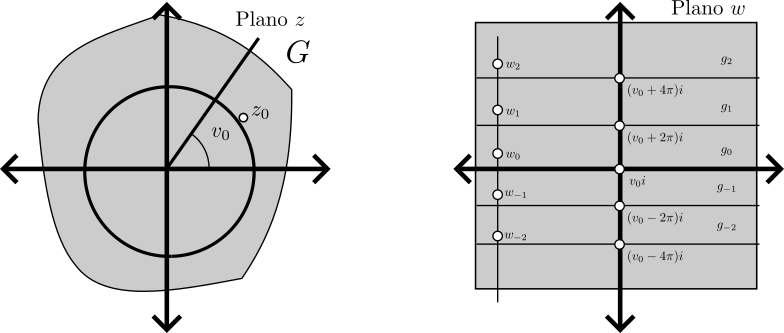
\includegraphics[width=0.7\linewidth]{img/log}
	\caption{Comportamiento del logaritmo complejo}
	\label{fig:log}
\end{figure}

Al igual que la función $w=z^\frac{1}{2}$ revierte el efecto de la función $w_1=z^2$, la función $f(z)=\ln z$ revierte el efecto de la función $g(z)=e^z$
\begin{mmaCell}{Input}
	 f[z_] = Log[z]\\polarConformal[f[r Exp[I*t]], \{r, 1, E\}, \{t, 0, 2 Pi\},\\Mesh -> \{30, 30\},LabelStyle -> Directive[Larger, Bold],\\PlotStyle -> White,MeshStyle -> Blue, Axes -> True,\\PlotRange -> \{\{-4, 4\}, \{-4, 4\}\}]
\end{mmaCell}
\begin{mmaCell}[moregraphics={moreig={scale=0.4}}]{Output}
	\mmaFrac{ \mmaGraphics{23.png}}{}
\end{mmaCell}
Como podemos ver en la imagen anterior, el logaritmo regresa el anillo $$\{z\in \C\mid 1<|z|<e\},$$ a la banda vertical $$\{z\in \C|\mbox{Re}(z)\in[0,1],\; \mbox{Im}(z)\in [-\pi,\pi]\}.$$

\section{Transformaciones de Möbius} \label{Möbius}

Comenzamos definiendo lo que es una transformación de Möbius
\begin{defi}
	Un mapeo de la forma 
	\begin{equation}\label{mobius}
		S(z)=\dfrac{az+b}{cz+d},
	\end{equation}
	 es llamada una transformación fraccional lineal. Si  además $a, b, c,$ y $d$ satisfacen que $ad-bc\neq 0$, entonces $S(z)$ es llamada una  transformación de Möbius.
\end{defi}

\begin{prop}\label{prop3}
	El mapeo $S(z)$, definido por la ecuación (\ref{mobius}), es biyectivo y conforme, de
	$$\Omega_{1}=\left\{z\in\C \left|\right. cz+d\neq 0\right\},$$
	sobre 
	$$\Omega_{2}=\left\{w\in\C \left|\right. w\neq \dfrac{a}{c}\right\}.$$
	De hecho, la inversa de $S(z)$ es también una transformación de Möbius dada por
	\begin{equation}\label{invMobius}
		S(w)=\dfrac{dw-b}{a-cw}.
	\end{equation}
Un bosquejo de demostración sería como sigue. Claramente$S(z)$ es analítica en $\Omega_{1}$ y $T(w) = (dw - b)/(a-cw)$ es
analítica en $\Omega_{2}$. El mapeo $S(z)$ será biyectivo si podemos mostrar que $T \circ S$ y $S \circ T$ son la función identidad, ya que esto significa que $S(z)$ tiene a $T(w)$ como su inversa. En efecto, esto se ve en estos cálculos:
\[
\begin{array}{ccl}
	S(T(w))&=&\dfrac{a\left(\dfrac{dw-b}{a-cw} \right) +b}{c\left(\dfrac{dw-b}{a-cw}\right)+d}\\
	&=&\dfrac{-adw+ab+bcw-ab}{-cdw+bc+dcw-da}\\
	&=&\dfrac{(bc-ad)w}{bc-ad}\\
	&=&w.
\end{array}
\]
Note que las cancelaciones realizadas son válidas pues $a-cw\neq  0$ y $bc-ad\neq 0$. Análogamente $T(S(z)) =z$.\\ 
Note que 
$$\dfrac{d}{dz}T(S(z))\dfrac{d}{dz}z=1,$$
y así $$T'(S(z))\cdot S'(z)=1.$$
Por lo tanto, $S'(z)\neq 0$.
\end{prop}
Sean $T(z)=\mobius{a}{+b}{c}{+d}$ y $S(z)=\mobius{e}{+f}{k}{+l}$ dos transformaciones de M\"obius, en Mathematica podemos definirlas como sigue

\begin{mmaCell}{Input}
	 T[z_] = (a z + b)/(c z + d);\\S[z_] = (ez + f)/(kz + l);
\end{mmaCell}
usando la instrucción \textbf{Simplify} podemos obtener la composición de las dos transformaciones de M\"obius anteriores  
\begin{mmaCell}{Input}
	 Simplify[T[S[z]]]
\end{mmaCell}
\begin{mmaCell}[moredefined={f, d}]{Input}
	 \mmaFrac{a f+b l+a e z+b k z}{c f+dl+c e z+d k z}
\end{mmaCell}
Acomodando los términos con el comando \textbf{Collect}
\begin{mmaCell}{Input}
	  Collect[Numerator[\%], z]/Collect[Denominator[\%], z]
\end{mmaCell}

\begin{mmaCell}[moredefined={f, d}]{Input}
    \mmaFrac{a f+b l+(a e+b k) z}{c f+d l+(c e+d k) z}
\end{mmaCell}
Lo anterior demuestra la siguiente 
\begin{prop}
	La composición de dos transformaciones de M\"obius es una transformación
	de M\"obius.
\end{prop}

De hecho, las transformaciones de M\"obius forman un grupo con la operación composición de funciones, recordemos la definición de grupo
\begin{defi}
	Sean $G$  un conjunto no vacío, y $*$ una operación binaria definida en $G$. Se dice que el par $( G , * )$ es un grupo si se cumplen las siguientes condiciones
	\begin{itemize}
		\item [1)] La operación $*$ verifica la propiedad asociativa: dados tres elementos cualesquiera de $g , h , k \in G$, se cumple que $$ (g* h)* k=g* (h*k).$$
		\item [2)] $G$ contiene un elemento distinguido llamado elemento neutro o identidad,6 denotado usualmente como $e$, con la siguiente propiedad: para cualquier $g\in G$
		$$e * g = g * e = g.$$ 
		\item [3)] Todo elemento $ g\in G$ tiene un elemento simétrico o inverso en el mismo  $G$, que se denota por $g^{-1}$, con la propiedad de que $$ g* g^{-1}=g^{-1}* g=e.$$
	\end{itemize}
\end{defi}

\begin{prop}
	El conjunto de transformaciones de M\"obius con la composición de funciones forman un grupo.\\
	Se dará un bosquejo de la demostración apoyándonos del cálculo simbólico de Mathematica. \\
	Sean $T(z)=\mobius{a}{+b}{c}{+d}$, $S(z)=\mobius{e}{+f}{k}{+l}$ y $R(z)=\mobius{m}{+n}{q}{+r}$  transformaciones de M\"obius
	
	\begin{mmaCell}{Input}
		T[z_] = (az + b)/(cz + d);\\S[z_] = (ez + f)/(kz + l);\\R[z_] = (mz + n)/(qz + r);
	\end{mmaCell}
	Realizando la composición $T(S(z))$ en Mathematica 
	\begin{mmaCell}{Input}
		Simplify[T[S[z]]]
	\end{mmaCell}
	\begin{mmaCell}[moredefined={f, d}]{Output}
		\mmaFrac{a f+b l+a e z+b k z}{c f+dl+c e z+d k z}
	\end{mmaCell}


definimos la composición $T(S(z))$ como \textbf{TS[z]}
\begin{mmaCell}[moredefined={f, d}]{Output}
	   TS[z_]=\mmaFrac{af+bl+aez+bkz}{cf+dl+cez+dkz}
\end{mmaCell}
\begin{mmaCell}{Input}
	  Simplify[TS[R[z]]];\\Collect[Numerator[\%], z]/Collect[Denominator[\%], z]
\end{mmaCell}

\begin{mmaCell}[moredefined={f}]{Output}
	   \mmaFrac{aen+bkn+afr+blr+(aem+bkm+afq+blq)z}{dkn+cen+dlr+cfr+(dkm+ce m+dlq+cfq)z}
\end{mmaCell}



por otro lado definimos la composición $S(R(z))$ como \textbf{TS[z]}
\begin{mmaCell}[moredefined={f, d}]{Output}
	  SR[z_]=\mmaFrac{e n+f r+e m z+f q z}{k n+l r+k m z+l q z}
\end{mmaCell}
\begin{mmaCell}{Input}
	 Simplify[T[SR[z]]];\\Collect[Numerator[\%], z]/Collect[Denominator[\%], z]
\end{mmaCell}
\begin{mmaCell}[moredefined={f}]{Output}
    \mmaFrac{aen+bkn+afr+blr+(aem+bkm+afq+blq)z}{dkn+cen+dlr+cfr+(dkm+ce m+dlq+cfq)z}
\end{mmaCell}
lo cual muestra que la operación composición es asociativa.\\
En Mathematica definimos el elemento neutro como
\begin{mmaCell}{Input}
	 Id[z_] = z;
\end{mmaCell}
Entonces 
\begin{mmaCell}{Input}
	 Simplify[Id[T[z]]]
\end{mmaCell}
\begin{mmaCell}{Output}
	 \mmaFrac{b+az}{d+cz}
\end{mmaCell}
análogamente 
\begin{mmaCell}{Input}
	 Simplify[T[Id[z]]]
\end{mmaCell}
\begin{mmaCell}{Output}
	 \mmaFrac{b+az}{d+cz}
\end{mmaCell}
Luego el elemento $Id(z)=z$ es el elemento neutro.\\
Consideremos la transformación $T_1(w)=\dfrac{-b+dw}{z-cw}$ 
\begin{mmaCell}{Input}
	  T1[w_]:=\mmaFrac{-b+dw}{z-cw}
\end{mmaCell}
Realizando la composición 

\begin{mmaCell}{Input}
	  Simplify[T[T1[w]]]
\end{mmaCell}
\begin{mmaCell}{Output}
	 w
\end{mmaCell}
de manera análoga 

\begin{mmaCell}{Input}
	 Simplify[T1[T[z]]]
\end{mmaCell}
\begin{mmaCell}{Output}
	 z
\end{mmaCell}
por tanto el conjunto de transformaciones de M\"obius con la composición de funciones forman un grupo.\endproof
\end{prop}
Sin embargo el grupo de las transformaciones de M\"obius  no es abeliano, por ejemplo tomemos las transformaciones
\[
	\begin{array}{ccl}
		T_1(z)=\dfrac{z}{z+1},&&T_2(z)=\dfrac{z+1}{z-1},
	\end{array}
\]
entonces 
\[
\begin{array}{ccl}
	T_1T_2(z)=\dfrac{z+1}{z},&&T_2T_1(z)=-2z-1,
\end{array}
\]

%%Ejemplo Möbius

\begin{Ejem}\label{ejemplo1}
	Sean $\Omega_{1}=\{x+iy\mid y>0;x,y\in \R\}$ y $\Omega_{2}=D(0,1)$, mostraremos que son conformemente equivalentes. Consideremos 
	$$f(z)=\dfrac{i-z}{i+z},$$
	para $z=x+iy\in\Omega_{1}$, entonces 
	$$f(z)=\dfrac{-x-i(y-1)}{x+i(y+1)},$$
	luego
	$$|f(z)|^2=f(z)\overline{f(z)}=\dfrac{x^2+(y-1)^2}{x^2+(y+1)^2},$$
	como $y>0$ se tiene que $f(z)\in\Omega_{2}$. Además, note que $f$ es analítica en $\Omega_{1}$ ya que $-i\notin\Omega_{1}$, también $f$ es inyectiva. Basta mostrar que $f$ es sobreyectiva.\\
	Sea $w\in\Omega_{2}$, escribamos $w=u+iv$ con $u^2+v^2<1$. Necesitamos encontrar $z\in\Omega_{1}$ tal que $f(z)=w$, es decir, $\dfrac{i-z}{i+z}=w$, resolviendo esta igualdad para $z$ obtenemos $z=i\left(\dfrac{1-w}{1+w}\right)$ y como $w=u+iv$ se tiene que 
	$$z=i\dfrac{(1-u-iv)(1+u-iv)}{(1+u+iv)(1+u+-iv)},$$
	por tanto $$\mbox{Im}(z)=\dfrac{1-u^2-v^2}{(1+u)^2+v^2}>0,$$
	y en consecuencia $z\in\Omega_{2}$.
\end{Ejem}
Las regiones $\Omega_{1}$ y $\Omega_{2}$ se grafican a continuación.
\begin{mmaCell}{Input}
	 omega1 = ComplexRegionPlot[Im[z] >= 0,\\ \{z, -5 - 5 I, 5 + 5 I\}, DisplayFunction -> Identity];
\end{mmaCell}

\begin{mmaCell}{Input}
	 omega2 =ComplexRegionPlot[ Im[I (1 - w)/(w + 1)] >= 0, \\ \{w, -1 - 1 I, 1 + 1 I \},DisplayFunction -> Identity ];
\end{mmaCell}

\begin{mmaCell}{Input}
	 Show[GraphicsGrid[\{\{Graphics[omega1], Graphics[omega2]\}\}, \\\{\}],DisplayFunction -> \$DisplayFunction]
\end{mmaCell}

\begin{mmaCell}[moregraphics={moreig={scale=0.4}}]{Output}
	\mmaFrac{ \mmaGraphics{9.png}}{}
\end{mmaCell}

Si queremos ver la imagen del semiplano superior bajo la función $f(z)=\dfrac{z-1}{z+1}$ que se discutió en el Ejemplo \ref{ejemplo1}, podemos hacerlo con \textbf{cartesianConformal}. Notemos que con esto solo obtenemos, en la imagen de la derecha, solo esa parte del círculo unitario asignada por el tamaño de la malla que en este caso usamos como parámetro \textbf{Mesh}$\rightarrow300$.
\begin{mmaCell}{Input}
	 cartesianConformal[w[x + I*y], \{x, -5, 5\}, \{y, 0, 5\},\\Mesh -> 300,LabelStyle ->Directive[Larger, Bold],\\PlotStyle -> White, MeshStyle -> Blue, Axes -> True,\\PlotPoints ->40, PlotRange -> All]
\end{mmaCell}
\begin{mmaCell}[moregraphics={moreig={scale=0.4}}]{Output}
	\mmaFrac{ \mmaGraphics{10.png}}{}
\end{mmaCell}
Recíprocamente, con la función inversa de $f$, $f^{-1}(z)=i\dfrac{z+1}{z-1}$ podemos ver como se transforma el círculo unitario en el semiplano superior. Para ello usaremos la función \textbf{polarConformal}. La instrucción \textbf{Mesh -> \{300, 300\}} nos indica que el círculo unitario se construirá a partir de 300 círculos concéntricos de radio menor que uno y 300 radios dentro del círculo.
\begin{mmaCell}{Input}
	  polarConformal[f[r Exp[I*t]], \{r, 0, 1\}, \{t, 0, 2 Pi\},\\Mesh -> \{300, 300\},LabelStyle -> Directive[Larger, Bold],\\PlotStyle -> White, MeshStyle -> Blue, Axes -> True]
\end{mmaCell}
\begin{mmaCell}[moregraphics={moreig={scale=0.4}}]{Output}
	\mmaFrac{ \mmaGraphics{11.png}}{}
\end{mmaCell}



\begin{defi}
	Sean $\alpha,\beta\in \C$ y $a,\theta\in\R$. Una función $w:\C\rightarrow\C$ se dice que es una 
	\begin{itemize}
		\item [1)] \textbf{Transformación lineal} si $w=\alpha z+\beta$.
		\item [2)] \textbf{Traslación} si $w=z+\beta$.
		\item [3)] \textbf{Estiramiento} si $w=az$.
		\item [4)] \textbf{Inversión} si $w=\dfrac{1}{z}$ si $z\neq0$.
		\item [5)] \textbf{Rotación} si $w=e^{i\theta}z$.
	\end{itemize}
\end{defi}
Estas funciones reciben el nombre de familia fundamental de transformaciones o transformaciones fundamentales.
\begin{Ejem}

Veamos el comportamiento gráfico de las  transformaciones fundamentales usando Mathematica, para ello consideraremos las siguientes transformaciones fundamentales:
\begin{itemize}
	\item [1)] si $w_1=(2-3i) z+ 5+i$,
	\item [2)] si $w_2=z+5+i$,
	\item [3)] si $w_3=4z$,
	\item [4)] si $w_4=\dfrac{1}{z}$ si $z\neq0$,
	\item [5)] si $w_5=e^{\frac{2}{3}\pi i}z$,
\end{itemize}
Usaremos la función \textbf{cartesianConformal} que ya se había construido previamente.
\begin{itemize}
	\item [1)] \begin{mmaCell}{Input}
		 W1[z_] = (2 - 3 I)*z + 5 + I\\cartesianConformal[W1[x + I*y], \{x, -5, 5\}, \{y, 0, 5\},\\Mesh -> 300, LabelStyle -> Directive[Larger, Bold],\\PlotStyle -> White,MeshStyle -> Blue, Axes -> True,\\PlotPoints -> 40,PlotRange -> All]
	\end{mmaCell}
	\begin{mmaCell}[moregraphics={moreig={scale=0.4}}]{Output}
		\mmaFrac{ \mmaGraphics{12.png}}{}
	\end{mmaCell}

	\item [2)] \begin{mmaCell}{Input}
		W2[z_] = z + 5 + I\\cartesianConformal[W2[x + I*y], \{x, -5, 5\}, \{y, 0, 5\},\\Mesh -> 300, LabelStyle -> Directive[Larger, Bold],\\PlotStyle -> White,MeshStyle -> Blue, Axes -> True,\\PlotPoints -> 40,PlotRange -> \{\{-10, 10\}, \{-10, 10\}\}]
	\end{mmaCell}
	\begin{mmaCell}[moregraphics={moreig={scale=0.4}}]{Output}
		\mmaFrac{ \mmaGraphics{13.png}}{}
	\end{mmaCell}

	\item [3)] \begin{mmaCell}{Input}
		W3[z_] = 4*z \\cartesianConformal[W3[x + I*y], \{x, -5, 5\}, \{y, 0, 5\},\\Mesh -> 300, LabelStyle -> Directive[Larger, Bold],\\PlotStyle -> White,MeshStyle -> Blue, Axes -> True,\\PlotPoints -> 40,PlotRange -> \{\{-30, 30\}, \{0, 30\}\}]
	\end{mmaCell}
	\begin{mmaCell}[moregraphics={moreig={scale=0.4}}]{Output}
		\mmaFrac{ \mmaGraphics{14.png}}{}
	\end{mmaCell}

	\item [4)] \begin{mmaCell}{Input}
		W4[z_] = 1/z \\cartesianConformal[W4[x + I*y], \{x, -5, 5\}, \{y, 0, 5\},\\Mesh -> 300, LabelStyle -> Directive[Larger, Bold],\\PlotStyle -> White,MeshStyle -> Blue, Axes -> True,\\PlotPoints -> 40,PlotRange ->\{\{-6, 6\}, \{-6, 6\}\}]
	\end{mmaCell}
	\begin{mmaCell}[moregraphics={moreig={scale=0.4}}]{Output}
		\mmaFrac{ \mmaGraphics{15.png}}{}
	\end{mmaCell}

	\item [5)] \begin{mmaCell}{Input}
		W5[z_] = Exp[2/3 * Pi *I]*z \\cartesianConformal[W5[x + I*y], \{x, -5, 5\}, \{y, 0, 5\},\\Mesh -> 300, LabelStyle -> Directive[Larger, Bold],\\PlotStyle -> White,MeshStyle -> Blue, Axes -> True,\\PlotPoints -> 40,PlotRange ->\{\{-7, 7\}, \{-7, 7\}\}]
	\end{mmaCell}
	\begin{mmaCell}[moregraphics={moreig={scale=0.4}}]{Output}
		\mmaFrac{ \mmaGraphics{16.png}}{}
	\end{mmaCell}
\end{itemize}
	
\end{Ejem}
Note que, gráficamente  una transformación de M\"obius se puede obtener a partir de aplicar distintas transformaciones fundamentales sucesivamente, formalmente 
\begin{prop}\label{prop4}
	Una transformación de M\"obius es la composición de transformaciones fundamentales.\\
	La prueba de esta proposición no es difícil, a continuación se da un esbozo de la demostración.\\ Sea $S(z)=\mobius{a}{+b}{c}{+d}$. Si $c=0$, entonces $S(z)=\dfrac{a}{d}z+\dfrac{b}{d}$, la cual es una transformación lineal.\\
	Si $c\neq 0$, entonces 
	\[
		\begin{array}{ccl}
			S(z)&=&\mobius{a}{+b}{c}{+d}\\
			&=&\dfrac{c^2(az+b)}{c^2(az+b)}\\
			&=&\dfrac{ac^2z + bc^2 + adc - adc}{c^2(az+b)}\\
			&=&\dfrac{ac(cz+d)+c(bc-ad)}{c^2(az+b)}\\
			&=&\dfrac{a}{c}+\dfrac{bc-ad}{c(cz+d)}\\
			&=&\alpha +\dfrac{\beta}{z+\gamma},
		\end{array}
	\]
	donde $\alpha=\dfrac{a}{c}$, $\beta=\dfrac{bc-ad}{c^2}$ y $\gamma=\dfrac{d}{c}$.\endproof
\end{prop}
El siguiente teorema es quizás, uno de los mas importantes en el análisis complejo pues establece, en palabras simples, que  todo subconjunto propio abierto sin agujeros del plano complejo se puede "meter" $\;$dentro de un disco abierto unitario. Este teorema fue enunciado  por Bernhard Riemann en 1851 en su tesis doctoral y aunque Riemann dio una prueba del teorema, esta no resulto ser correcta, no fue sino hasta 1900 cuando William Fogg Osgood dio la primera demostración rigurosa del teorema.

\begin{teor}[del mapeo de Riemann]\label{TMR}
	Sea $\Omega$ una región simplemente conexa tal que $\Omega\neq \C$. Entonces existe un mapeo conforme biyectivo $f: \Omega\rightarrow D$, donde $D =\{ z : |z| < 1 \}$.\\
	La demostración se puede consultar en \cite{tarlok} página 85, Teorema 3.10.
\end{teor}
Bajo ciertas condiciones la función que se enuncia en el Teorema \ref{TMR} es única
\begin{prop}\label{propTMR}
 Asuma que $\Omega$ satisface las suposiciones del Teorema \ref{TMR} y sea $z_0\in \Omega$. Entonces existe una única función $f:\Omega\rightarrow D$ tal que  $f\in \mathcal{H}(\Omega)$, $f$ es inyectiva y $f(z_0)$ con $f'(z_0)>0$.\\
 La demostración se puede consultar en el Teorema 3.18 página 94 de \cite{tarlok}.
\end{prop}

\begin{coro}\label{coroRiemman}
	 Asuma que $\Omega$ satisface las suposiciones del Teorema \ref{TMR} y sean $z_0\in \Omega$, $w_0\in D$ y un ángulo $\theta_0$ y al asumir la Proposición \ref{propTMR}, demuestre que existe un mapeo conforme $f:\Omega\rightarrow D$ tal que $f(z_0)=w_0$ y $\mbox{arg}f'(z_0)=\theta_0$, y además $f$ es único.
\end{coro}

\begin{teor}[del módulo máximo]\label{modmx}
	Suponga que $f (z)$ es analítica en el interior y sobre una curva simple cerrada $C$. Así, el valor máximo de $| f (z)|$ se encuentra sobre $C$, a menos que $f (z)$ sea una constante.\\
	La demostración se puede consultar en \cite{marsden}, es el Teorema 6.3.5 de dicha referencia.
\end{teor}
\begin{prop}
	Cualquier mapeo conforme de $D =\{ z : |z| < 1 \}$ sobre sí mismo es un mapeo de la forma de la forma
	$$T(z)=e^{i\theta}\dfrac{z-z_{0}}{1-\bar{z_{0}}z},$$
	para alguna $z_{0}\in D$ fija y $\theta \in [0, 2\pi[$; más aún, cualquier $T$ de esta forma es un mapeo conforme de $D$ sobre $D$, y además $T$ es único.\\
	La demostración la podemos consultar en \cite{marsden}, vea la Proposición  5.2.2.

\end{prop}
Notemos que, la transformación lineal entera $w = az+b$ $(a\neq 0)$ claramente preserva círculos, ya que el mapeo $w$ es solo una traslación  (si $a = 1)$, o una traslación combinada con un estiramiento (si $a\neq 1$).
\begin{lema}\label{lema1}
	La transformación
	$$w=\dfrac{1}{z},$$
	preserva círculos.\\
Una forma de probar el lema anterior es usar la proyección estereográfica y utilizar el hecho de que esta manda rectas o círculos del plano en círculos de la esfera y
que la inversa manda círculos de la esfera en rectas o círculos del plano. Un bosquejo de la demostración sería como sigue.\\
Sea $\pi(z)=(x_1,x_2,x_3)$ un punto de la esfera $S^2$ , tomemos $z=x+iy$ en el plano $Z$ y $w=\dfrac{1}{z}=\dfrac{\overline{z}}{z\overline{z}}=\dfrac{x-iy}{x^2+y^2}$ en el plano $W$. Tenemos que 
$$|w|^2=\dfrac{1}{x^2+y^2}\implies |w|^2+1=\dfrac{x^2+y^2+1}{x^2+y^2}.$$
Utilizando las coordenadas en la esfera el punto $w$ se tiene 
$$y_1=\dfrac{w+\overline{w}}{1+|w|^2}=\dfrac{2x}{|z|^2+1}=x_1,$$
$$y_1=\dfrac{w-\overline{w}}{i(|w|^2+1)}=-\dfrac{2iy}{i(|z|^1+1)}=-x_2,$$
$$y_3=\dfrac{|w|^2-1}{|w|^2+1}=\dfrac{1-|z|^2}{1+|z|^2}=-x_3,$$
es decir, si miramos a $w=\dfrac{1}{z}$ como la acción bajo la proyección estereográfica, $w$ vista en la esfera deja fija la coordenada $x_1$, luego es una rotación de $x_2$ a $-x_2$ y otra rotación  de $x_3$ a $-x_3$, ambas acciones preservan círculos en la esfera. De aquí se sigue el resultado
\end{lema}

\begin{prop}
	Toda transformación de M\"obius 
	\begin{equation}\label{trmob}
		T(z)=w=\mobius{a}{+b}{c}{+d},
	\end{equation}
	preserva círculos.\\
	La prueba de esta proposición es consecuencia del Lema \ref{lema1}, a continuación, se da un bosquejo.\\
	Si $c=0$ es resultado es claro. Consideremos el caso cuando $c\neq0$, entonces $w$ se puede escribir de la forma 
	$$w=\dfrac{a}{c}+\dfrac{bc-ad}{c(cz+d)},$$
	si $z_1=L_1(z)=cz+d$ y $z_2=L_2=\dfrac{1}{z_1}$ entonces 
	$$L_3(z_2)=\dfrac{a}{c}+\dfrac{bc-ad}{c}z_2,$$
	luego $w$ se puede escribir como el producto $$w=L_3L_2L_1,$$ de tres transformaciones que preservan círculos. Luego $T$ preserva círculos.
\end{prop}
\begin{coro}
	Sea $\delta=-\dfrac{d}{c}$ el polo de la transformación de M\"obius $$T(z)=w=\mobius{a}{+b}{c}{+d}.$$ Entonces la transformación $T$ mapea toda recta o círculo que pasa a través de $\delta$ en una recta,  y cualquier otra línea recta o círculo en un circulo.
\end{coro}
Consideremos la transformación de M\"obius $$T(z)=\mobius{5}{+(5+3i)}{(2.4+3.2i)}{+{4.3+7.2i}}$$
y el disco $D=\{z\in \C: |z|< 1\}$
Podemos usar la función \textbf{polarConformal} para comprobar visualmente la proposición anterior
\begin{mmaCell}{Input}
	 TMobius[z_, a_, b_, c_, d_] = (a*z + b)/(c*z + d);\\polarConformal[ TMobius[r Exp[I*t], 5, 5 + 3 I,\\2.4 + 3.2 I, 4.3 + 7.2 I],\\\{r, 0, 1\}, \{t, 0, 2 Pi\},Mesh->\{0, 0\},\\PlotRange ->Automatic,LabelStyle-> Directive[Larger,Bold],\\PlotStyle -> White,MeshStyle -> Blue, Axes -> True]
\end{mmaCell}
\begin{mmaCell}[moregraphics={moreig={scale=0.4}}]{Output}
	\mmaFrac{ \mmaGraphics{27.png}}{}
\end{mmaCell}

Consideremos los puntos $z_{1}, z_{2}, z_{3}$ en el plano $z$ y respectivamente los puntos $w_{1}, w_{2}, w_{3}$ en el plano $W$. Si $w_k$ corresponde a $z_k$, $k=1,2,3$, se tiene 
$$w-w_k=\mobius{a}{+b}{c}{+d}-\dfrac{az_k+b}{cz_k+d}=\dfrac{(ad-bc)(z-z_k)}{(cz+d)(cz_k+d)},$$
así que 
\[
	\begin{array}{cc}
		w-w_1=\dfrac{(ad-bc)(z-z_1)}{(cz+d)(cz_1+d)},&w-w_3=\dfrac{(ad-bc)(z-z_3)}{(cz+d)(cz_3+d)},
	\end{array}
\]
Sustituyendo $w$ por $w_2$ y $z$ por $z_2$,
\[
\begin{array}{cc}
	w_2-w_1=\dfrac{(ad-bc)(z_2-z_1)}{(cz_2+d)(cz_1+d)},&w_2-w_3=\dfrac{(ad-bc)(z_2-z_3)}{(cz_2+d)(cz_3+d)}.
\end{array}
\]
Si suponemos que $ad-bc\neq 0$, entonces 
\begin{equation}\label{razoncruzada}
	\dfrac{(w-w_1)(w_2-w_3)}{(w-w_3)(w_2-w_1)}=\dfrac{(z-z_1)(z_2-z_3)}{(z-z_3)(z_2-z_1)}.
\end{equation}
Si se despeja $w$ en términos de $z$ y se obtiene una transformación de M\"obius $S$ que manda $z_i \rightarrow w_i$, $i = l , 2, 3$. Se ha demostrado la siguiente
\begin{prop}[Razón cruzada]
	Dados dos conjuntos de puntos distintos $z_{1}, z_{2}, z_{3}$ y $w_{1}, w_{2}, w_{3}$, existe una única transformación de M\"obius $S$ que manda $z_i \rightarrow w_i$, $i = l , 2, 3$, De hecho, si $S(z) = w$, entonces $$\dfrac{(w-w_1)(w_2-w_3)}{(w-w_3)(w_2-w_1)}=\dfrac{(z-z_1)(z_2-z_3)}{(z-z_3)(z_2-z_1)}.$$
\end{prop}
\subsection{Transformaciones de M\"obius en el plano extendido}

Consideremos la transformación 
\begin{equation}\label{mob}
	w=\mobius{a}{+b}{c}{+d},
\end{equation} 
Cuando un punto $w$ es la imagen de algún punto $z$ bajo la transformación (\ref{mob}), el punto $z$ se recupera por medio de la transformación (\ref{invMobius}).\\
Si $c=0$, de modo que $a\neq 0$, $d\neq 0$, cada punto en el plano $W$ es la imagen de uno y solo un punto en el plano $Z$. Lo mismo es cierto si  $c\neq 0$, excepto cuando $w=\dfrac{a}{c}$ ya que el denominador de la ecuación (\ref{invMobius}) se anula si $w$ tiene ese valor, sin embargo, podemos ampliar el dominio que se dio en la Proposición \ref{prop3} para las trasformaciones de M\"obius para definir una trasformación de M\"obius  en el plano extendido
$$\bar{\C}=\C\cup \{\infty\},$$
tal que el punto $w=\dfrac{a}{c}$ es la imagen de $z=\infty$ cuando $c\neq 0$, la definición de esta transformación sería la siguiente 

\[
	S(z)=\left\{ \begin{array}{ccl}
		\mobius{a}{+b}{c}{+d},& &\mbox{ si } z\in \C\setminus\left\{-\dfrac{d}{c}\right\}\\\\
		\dfrac{a}{c},& &\mbox{ si } z=\infty\\\\
		\infty,& &\mbox{ si } z=-\dfrac{d}{c},
	\end{array} \right.
\]
y si $c=0$, 
\[
S(z)=\left\{ \begin{array}{ccl}
	\dfrac{a}{d}z+\dfrac{b}{d},& &\mbox{ si } z\in \C\\
	\infty,& &\mbox{ si } z=\infty,
\end{array} \right.
\]
No es difícil ver que los siguientes límites se cumplen
\[
\begin{array}{ccl}
	\ds\lim_{z\rightarrow\infty}S(z)= \infty,&&\mbox{ si } c=0,\\
	\ds\lim_{z\rightarrow\infty}S(z)= \dfrac{a}{c},&&\mbox{ si } c\neq0,\\
	\ds\lim_{z\rightarrow -\dfrac{d}{c}}S(z)= \infty,&&\mbox{ si } c\neq 0,
\end{array}
\] 
lo cual muestra que las transformaciones de M\"obius definidas de esta forma son continuas en el plano extendido. Asimismo, en el plano extendido las transformaciones definidas ahí también resultan ser biyecciones. Por lo tanto, podemos habar de la transformación de M\"obius inversa
definida de la siguiente forma

\[
S^{-1}(w)=\left\{ \begin{array}{ccl}
	\infty,& &\mbox{ si } w=\infty \mbox{ y } c=0\\
	\infty,& &\mbox{ si } w=\dfrac{a}{c} \mbox{ y } c\neq0\\
	-\dfrac{d}{c},& &\mbox{ si } w=\infty \mbox{ y } c\neq0.
\end{array} \right.
\]
\begin{Ejem}
	Considere los puntos $z_1=1$, $z_2=0$, $z_3=-1$ y $w_1=i$, $w_2=\infty$, $w_3=1$, en este caso la fórmula de la razón cruzada quedaría de la siguiente manera
	$$\dfrac{w-w_1}{w-w_3}=\dfrac{(z-z_1)(z_2-z_3)}{(z-z_3)(z_2-z_1)},$$
	sustituyendo valores quedaría como
	$$\dfrac{w-i}{w-1}=\dfrac{(z-1)(0+1)}{(z+1)(0-1)},$$
	despejando para $w$ se obtiene 
	$$w=\dfrac{(i+1)z+(i-1)}{2z},$$
\end{Ejem}
A continuación implementamos el método de la razón cruzada en Mathematica
\begin{mmaCell}{Input}
	 Mobius[z_, a_, b_, c_, d_] := (a z + b)/(c z + d)\\
\end{mmaCell}
\begin{mmaCell}{Input}
	 Clear[RazonCruzada, za, zb, zc, wa, wb, wc]\\RazonCruzada[z_, \{za_, zb_, zc_\}, \{wa_, wb_, wc_\}] :=\\Module[\{soln\},soln = Solve[\{wa == Mobius[za, a, b, c, 1],\\wb == Mobius[zb, a, b, c, 1], wc == Mobius[zc,a,b,c,1]\},\\\{a,b,c\}];\\Mobius[z, a, b, c, 1] /. soln[[1]]]
\end{mmaCell}
Consideremos nuevamente los puntos $z_1=1$, $z_2=0$, $z_3=-1$ y $w_1=i$, $w_2=\infty$, $w_3=1$ pero esta vez $w_2= t$ y aplicaremos el límite cuando $t\rightarrow\infty$
\begin{mmaCell}{Input}
	   RazonCruzada[z, {1, 0, -1}, {I, t, 1}]
\end{mmaCell}
\begin{mmaCell}[moredefined={t}]{Output}
	  \mmaFrac{t-i ((-1-i)+t) z}{1+(i-(1+i) t) z}
\end{mmaCell}
Tomando el límite 
\begin{mmaCell}[moredefined={t}]{Input}
	 Limit[\mmaFrac{t-i ((-1-i)+t) z}{1+(i-(1+i) t) z},t -> Infinity]\\Collect[Numerator[%], z]/Collect[Denominator[%], z]
\end{mmaCell}
\begin{mmaCell}{Input}
	 \mmaFrac{(-1+i)+(1+i) z}{2 z}
\end{mmaCell}

\section{Mapeo de Joukowski} \label{Joukowski}


\begin{Ejem}
	Encuentre las líneas de corriente para el flujo alrededor de un obstáculo cilíndrico centrado en el origen y de radio $R$.
	\solu
	Por un momento supongamos que el flujo es simétrico con respecto al eje $x$. Basta estudiar el flujo cuando $y\geq 0$. Para mapear la región de flujo en el semiplano superior necesitamos una función analítica $f(z)$ que sea real al menos para $|x|>R$ y en el círculo $|z|=R$. La primera condición se cumple para las funciones racionales con coeficientes reales, para la segunda condición notemos que el círculo puede ser descrito por
	$$z\bar{z}=R^2,$$
	se tiene así que $\bar{z}=\dfrac{R^2}{z}$, por lo tanto la función racional $z+\dfrac{R^2}{z}$ es igual a $z+\bar{z}="\mbox{Re}z$  en el círculo, en consecuencia tenemos el mapeo
	$$w=f(z)=z+\dfrac{R^2}{z}.$$
	Esta función es un mapeo inyectivo de la región de flujo para $y>0$ sobre el semiplano superior. Por lo tanto, la función de flujo apropiada corresponde a $\psi(u, v) = v = \mbox{Im}w$, dando las líneas de corriente
	$$\varphi(x,y)=\mbox{Im}\left(z+\dfrac{R^2}{z}\right)=\mbox{cte}.$$\endproof
	
\end{Ejem}



Si eliminamos el supuesto que el flujo sea simétrico, entonces solo requerimos que el círculo mismo sea una línea de corriente. Por lo tanto podemos agregar cualquier múltiplo constante  de $\log |z|$ (ya que se tiene que $|z|=R$ es una línea de corriente) a la función de corriente y obtener los patrones de flujo circulante.\\

En 1908 el matemático Nikolái Zhukovski  (a veces escrito Joukowski) estudio este tipo de mapeos pero no aplicados al círculo $|z|=R$, si no a círculos $C$ cuyo centro fuera distinto al origen. El resultado que obtuvo fue un perfil aerodinámico como el de la figura \ref{fig:24}.\\Al comenzar con diferentes círculos C, podemos generar una variedad de estos llamados perfiles aerodinámicos de Joukowski, podemos usar la transformación de Joukowski para calcular los flujos alrededor de distintos perfiles aerodinámicos. Por ejemplo, podemos dar forma al perfil aerodinámico para cumplir con ciertas especificaciones de ingeniería eligiendo adecuadamente $C$ e introduciendo modificaciones en el mapeo como, por ejemplo:
$$w=f(z)=z+\dfrac{R^2}{z}+\dfrac{a}{z^2}+\dfrac{b}{z^2}+\cdots$$
\begin{figure}[h!]
	\centering
	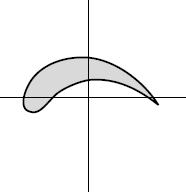
\includegraphics[width=0.2\linewidth]{img/24}
	\caption{Perfil aerodinámico}
	\label{fig:24}
\end{figure}
 

Consideremos ahora el mapeo 
\begin{equation}
	w=J(z)=\dfrac{1}{2}\left(z+\dfrac{1}{z}\right)=\dfrac{z^2+1}{2z},
\end{equation}
no es difícil ver que 
\begin{equation}\label{derj}
	J(z)=J\left(\dfrac{1}{z}\right).
\end{equation}
Además tenemos que $J(0)=J(\infty)=\infty$. \\
Derivando obtenemos $$J'(z)=\dfrac{1}{2}\left(z-\dfrac{1}{z^2}\right).$$
Luego $J'(z)=0$, si y sólo si, $z=\pm 1$, por lo que $J$ es conforme en $\C\setminus\{0,\pm 1\}$. Por otro lado, si $J(z_1)=J(z_2)$ entonces $z_{1}^2z_2+z_2=z_{2}^2+z_1$, luego $(z_1-z_2)(z_1z_2-1)=0$ de donde $z_1=z_2$ o $z_1z_2=1$, es decir, que cada punto del plano $W$ tiene en la transformación $w$ dos preimágenes $z_1$ y $z_2$ ligadas por la relación $z_1z_2=1$. Si una de éstas preimágenes pertenece al interior del círculo unitario, la otra pertenece al exterior  y viceversa. A continuación, veremos como el mapeo $J(z)$ transforma dominio $D=\{z\in \C\mid |z|\leq 1 \}$ en un dominio $G$ de del plano $W$ muy parecido a un perfil aerodinámico. Veamos primero la imagen de la frontera de $D$, $$\partial D=\{z\in\C\mid |z|=1\}.$$
Si $z=e^{it}$, con $t\in[0,2\pi]$, entonces $J(e^{it})=\dfrac{1}{2}\left(e^{it}+e^{-it}\right)=\cos t$, es decir, la imagen de $\partial D$ bajo $J$ es el segmento del eje real $[-1,1]$ recorrido dos veces. Por lo que, se puede afirmar que $G$ está formado por todos aquellos puntos del plano $W$  a excepción de aquellos que pertenecen al segmento del eje real $[-1,1]$. En efecto, consideremos las imágenes de las circunferencias $|z|=r$ y los radios $\mbox{Arg}\; z=\alpha+2k\pi$, consideremos solo el interior de $D$, $(D^{\circ})$. Tomando el cambio $z=re^{it}$ con $t\in[0,2\pi]$ y $r\in (0,1)$, entonces
$$J(z)=J(re^{it})=\dfrac{1}{2}\left(r+\dfrac{1}{r}\right)\cos t-i\dfrac{1}{2}\left(\dfrac{1}{r}-r\right)\sen t,$$
o bien 
$$u=\dfrac{1}{2}\left(r+\dfrac{1}{r}\right)\cos t,$$
$$v=\dfrac{1}{2}\left(r-\dfrac{1}{r}\right)\sen t,$$
de donde obtenemos 
\begin{equation}\label{ecelip}
	\dfrac{u^2}{\left[\dfrac{1}{2}\left(r+\dfrac{1}{r}\right)\right]^2} +\dfrac{v^2}{\left[\dfrac{1}{2}\left(\dfrac{1}{r}-r\right)\right]^2}=1.
\end{equation}
Esta es la ecuación de una elipse con los semiejes $a=\dfrac{1}{2}\left(r+\dfrac{1}{r}\right)$ y $b=\dfrac{1}{2}\left(\dfrac{1}{r}-r\right)$; y los focos $\pm 1$. De las ecuaciones para $u$ y $v$; y (\ref{ecelip}) se deduce que, cuando $t$ crece continuamente desde $0$ hasta $2\pi$, el punto correspondiente describe una vez la elipse (\ref{ecelip}) en dirección negativa. En efecto, cuando $t\in[0,\frac{\pi}{2}]$, $u$ es positivo y decrece desde $a$ hasta $0$, mientras que $v$ es negativo y decrece desde $0$ hasta $-b$; cuando $t\in(\frac{\pi}{2},\pi)$, $u$ continúa decreciendo desde $0$ hasta $-a$, mientras que $v$ decrece desde $-b$ hasta $0$; cuando $t\in (\pi ,\frac{3\pi}{2})$, $u$ crece desde $-a$ hasta $0$, mientras que $v$ crece desde $0$ hasta $b$; finalmente, cuando $t\in (\frac{3\pi}{2},2\pi)$, $u$ crece desde $0$ hasta $a$, mientras que $v$ decrece desde $b$ hasta $0$.\\
Variando el radio $r$ de la circunferencia $|z|=1$ desde $0$ hasta $1$, hacemos decrecer a $a$ desde $\infty$ hasta $1$ y $b$, desde $\infty$ a $0$; las elipses correspondientes describirán todo el conjunto de elipses del plano $W$ con los focos $\pm 1$. De aquí se deduce que $J(z)$ transforma biunívocamente  el círculo unitario es el conjunto $G$ que representa el exterior del segmento $[-1,1]$.\\
Para la imagen del radio $z=te^{i\alpha}$, $t\in[0,1]$, primero obtenemos la ecuación 
\begin{equation}\label{echip}
	J(z)=\dfrac{1}{2}\left(\dfrac{1}{t}+t\right)\cos \alpha-i\dfrac{1}{2}\left(\dfrac{1}{t}-t\right)\sen \alpha,
\end{equation}
de donde 
$$u=\dfrac{1}{2}\left(\dfrac{1}{t}+t\right)\cos \alpha,$$
$$v=-\dfrac{1}{2}\left(\dfrac{1}{t}-t\right)\sen \alpha,$$
de aquí vemos que las imágenes de dos radios, simétricos respecto del eje real, también son simétricos respectos del eje real, mientras que las imágenes de dos radios, simétricos respecto del eje imaginario, son simétricos respecto al eje imaginario. Es por ello que basta considerar solamente la imágenes de los radios pertenecientes al cuadrante $0\leq \alpha\leq \dfrac{\pi}{2}$.\\
Para $\alpha=0$ tenemos 
$$u=0,$$
$$v=-\dfrac{1}{2}\left(\dfrac{1}{t}-t\right),$$
con $t\in[0,1]$. Estos es un subintervalo infinito del eje real: $1<u<\infty$. El intervalo simétrico a éste $-\infty<u<-1$ es la imagen del radio que corresponde a $\alpha=\pi$.\\
Para $\alpha=\dfrac{\pi}{2}$, se tiene: 
$$u=0,$$
$$v=-\dfrac{1}{2}\left(\dfrac{1}{t}-t\right),$$
con $t\in[0,1]$. Este es el semieje imaginario $-\infty<v<0$. El otro semieje imaginario $0<v<\infty$ es la imagen del radio que corresponde a $\alpha=-\dfrac{\pi}{2}$.\\
Supongamos ahora que $0<\alpha<\dfrac{\pi}{2}$. Entonces de las ecuaciones para $u,v$ y (\ref{echip}) se obtiene
\begin{equation}\label{elipse}
	\dfrac{u^2}{\cos^{2}\alpha}-\dfrac{v^2}{\sen^{2}\alpha}=1.
\end{equation}
Esta es la ecuación de una hipérbola $H$ con el semieje real $a=\cos \alpha$; con semieje imaginario $b=\sen \alpha$ y con los focos $\pm 1$. Sea $H_k$ la intersección de $H$ con el $i$-ésimo cuadrante para cada $i=1,2,3,4$ respectivamente, excluyendo los puntos $(\pm a,0)$ de $H$ que pertenecen al eje real. Además, sean $R_{\alpha}$, $R_{\pi-\alpha}$, $R_{\pi+\alpha}$ y $R_{-\alpha}$ los conjuntos de puntos que pertenecen al radio $z=te^{i\alpha}$ con inclinaciones $\alpha$, $\pi-\alpha$, $\pi +\alpha$ y $-\alpha$ respectivamente. Tenemos que 
\[
	\begin{array}{cccc}
		H_1=J(R_{-\alpha}),&H_2=J(R_{\pi + \alpha}),&H_3=J(R_{\pi -\alpha}), &H_4=J(R_{\alpha}).
	\end{array}
\]
Note que la imagen de cada uno de los diámetros formados por estos radios será la parte de la $H$ formada por los pares de sus cuartas partes que son simétricas respecto del origen de coordenadas y que están ligadas entre sí en el punto del infinito.\\
Resumiendo, la función $J(z)$ transforma biunívocamente tanto el interior como el exterior del círculo unidad en el exterior del segmento $-1\leq u \leq 1$ (del eje real).  En este caso, las circunferencias $|z|=r$ se transforman en elipses con los focos $\pm1$ y semiejes $\dfrac{1}{2}\left|\dfrac{1}{r}\pm r \right|$, y los pares de diámetros simétricos respecto de los ejes coordenados formados por los radios $z=\pm re^{i\alpha}$ donde $0<\alpha<\dfrac{\pi}{2}$ se transforman en hipérbolas con los focos $\pm 1$ y semiejes $|\cos\alpha|$, $|\sen\alpha|$ a excepción de los vértices de estas hipérbolas. 

\subsection{Mapeo de Joukowski usando Mathematica} \label{Joukowski-mathematica}
La siguiente implementación en Mathematica se tomo de \cite{GeometryJo}.

\begin{mmaCell}{Input}
	 rotationTransform[\mmaPat{\(\pmb{\zeta}\)_},\mmaPat{\(\pmb{\alpha}\)_}]:=\mmaPat{\(\pmb{\zeta}\)} \mmaSup{\mmaDef{e}}{\mmaDef{i} \mmaPat{\(\pmb{\alpha}\)}}
\end{mmaCell}

\begin{mmaCell}[moredefined={translationTransform}]{Input}
	 translationTransform[\mmaPat{\(\pmb{\zeta}\)_},\mmaPat{\(\pmb{\mu}\)_}]:=\mmaPat{\(\pmb{\zeta}\)}+\mmaPat{\(\pmb{\mu}\)}
\end{mmaCell}
\begin{mmaCell}[moredefined={joukowskiTransform}]{Input}
	 joukowskiTransform[\mmaPat{\(\pmb{\zeta}\)_}]:=0.5* (\mmaPat{\(\pmb{\zeta}\)}+\mmaFrac{1}{\mmaPat{\(\pmb{\zeta}\)}})
\end{mmaCell}
\begin{mmaCell}{Input}
	 Function[\mmaPat{\(\pmb{\zeta}\)},0.5*(\mmaPat{\(\pmb{\zeta}\)}+\mmaFrac{1}{\mmaPat{\(\pmb{\zeta}\)}})]
\end{mmaCell}
\begin{mmaCell}[morelocal={a}]{Input}
	 \mmaDef{\(\pmb{\zeta}\)0C}[\mmaPat{\(\pmb{\theta}\)_},\mmaPat{\(\pmb{\mu}\)_}]:=Module[\{a,\mmaLoc{\(\pmb{\beta}\)}\},\{a,\mmaLoc{\(\pmb{\beta}\)}\}=\{Abs[1-\mmaPat{\(\pmb{\mu}\)}],-Arg[1-\mmaPat{\(\pmb{\mu}\)}]\};\\a \mmaSup{\mmaDef{e}}{-\mmaDef{i} (\mmaPat{\(\pmb{\theta}\)}+\mmaLoc{\(\pmb{\beta}\)})}]
\end{mmaCell}
\begin{mmaCell}[moredefined={translationTransform}]{Input}
	 \mmaDef{\(\pmb{\zeta}\)C}[\mmaPat{\(\pmb{\theta}\)_},\mmaPat{\(\pmb{\mu}\)_}]:=translationTransform[\mmaDef{\(\pmb{\zeta}\)0C}[\mmaPat{\(\pmb{\theta}\)},\mmaPat{\(\pmb{\mu}\)}],\mmaPat{\(\pmb{\mu}\)}]
\end{mmaCell}
\begin{mmaCell}[moredefined={zA, joukowskiTransform}]{Input}
	 zA[\mmaPat{\(\pmb{\theta}\)_},\mmaPat{\(\pmb{\mu}\)_}]:=joukowskiTransform[\mmaDef{\(\pmb{\zeta}\)C}[\mmaPat{\(\pmb{\theta}\)},\mmaPat{\(\pmb{\mu}\)}]]
\end{mmaCell}
\begin{mmaCell}[moredefined={zA}]{Input}
	\mmaDef{\(\pmb{\theta}\)LE}[\mmaPat{\(\pmb{\mu}\)_}]:=\mmaUnd{\(\pmb{\theta}\)}/.\(\pmb{\,}\)FindRoot[Im[zA[\mmaFnc{\(\pmb{\theta}\)},\mmaPat{\(\pmb{\mu}\)}]],\{\mmaFnc{\(\pmb{\theta}\)},\mmaDef{\(\pmb{\pi}\)}\}]
\end{mmaCell}

\begin{mmaCell}[moredefined={xLE, zA}]{Input}
	xLE[\mmaPat{\(\pmb{\mu}\)_}]:=Chop[zA[\mmaDef{\(\pmb{\theta}\)LE}[\mmaPat{\(\pmb{\mu}\)}],\mmaPat{\(\pmb{\mu}\)}]]
\end{mmaCell}

\begin{mmaCell}[moredefined={xLE, zA}]{Input}
	 Manipulate[\\Module[\{a,c,gz,gzA,gzCrit,\mmaUnd{g\(\pmb{\zeta}\)},\mmaUnd{g\(\pmb{\zeta}\)C},\\\mmaUnd{g\(\pmb{\zeta}\)Crit},\mmaUnd{g\(\pmb{\zeta}\)Tri},za,\mmaUnd{\(\pmb{\zeta}\)c},\mmaUnd{\(\pmb{\beta}\)},\mmaUnd{\(\pmb{\mu}\)}\},\\\{\mmaUnd{\(\pmb{\mu}\)},a,\mmaUnd{\(\pmb{\beta}\)}\}=\{r\mmaSup{\mmaDef{e}}{\mmaDef{i}\mmaUnd{\(\pmb{\alpha}\)}},Abs[1-\mmaUnd{\(\pmb{\mu}\)}],-Arg[1-\mmaUnd{\(\pmb{\mu}\)}]\};\\\mmaUnd{\(\pmb{\mu}\)}=r\mmaSup{\mmaDef{e}}{\mmaDef{i}\mmaUnd{\(\pmb{\alpha}\)}}(*translation vector as complex number*);\\a=Abs[1-\mmaUnd{\(\pmb{\mu}\)}](*radius of circle forcing circle to pass \\through \(\pmb{\zeta}\)=1*);\\\mmaUnd{\(\pmb{\beta}\)}=-Arg[1-\mmaUnd{\(\pmb{\mu}\)}](*angle in reference triangle opposite side \(\pmb{\mu}\)*);\\(* complex plane of circle *)\\\mmaUnd{\(\pmb{\zeta}\)c}=\mmaDef{\(\pmb{\zeta}\)C}[\mmaUnd{\(\pmb{\theta}\)},\mmaUnd{\(\pmb{\mu}\)}];\\\mmaUnd{g\(\pmb{\zeta}\)C}=ParametricPlot[\{Re[\mmaUnd{\(\pmb{\zeta}\)c}],Im[\mmaUnd{\(\pmb{\zeta}\)c}]\},\{\mmaFnc{\(\pmb{\theta}\)},0,2\mmaDef{\(\pmb{\pi}\)}\},PlotStyle\\\(\pmb{\to}\)\{Thick,Black\}];\\\mmaUnd{g\(\pmb{\zeta}\)Tri}=Graphics[\{EdgeForm[Thin],Polygon[\{\{0,0\},\\\{Re[\mmaUnd{\(\pmb{\mu}\)}],Im[\mmaUnd{\(\pmb{\mu}\)}]\},\{1,0\}\}]\}];\\\mmaUnd{g\(\pmb{\zeta}\)Crit}=Graphics[\{Black,PointSize[Medium],Point[\{\{1,0\},\\\{-1,0\}\}]\}];\\\mmaUnd{g\(\pmb{\zeta}\)}=Show[\mmaUnd{g\(\pmb{\zeta}\)C},\mmaUnd{g\(\pmb{\zeta}\)Tri},\mmaUnd{g\(\pmb{\zeta}\)Crit},Axes\(\pmb{\to}\)None,Frame\(\pmb{\to}\)True,\\FrameLabel \(\pmb{\to}\)\{\{x,None\},\{y,"plano z"\}\},ImageSize\(\pmb{\to}\)3.95 72,\\PlotRange\(\pmb{\to}\)3,RotateLabel\(\pmb{\to}\)False];\\(* complex plane of airfoil *)\\za=zA[\mmaUnd{\(\pmb{\theta}\)},\mmaUnd{\(\pmb{\mu}\)}];\\c=2-xLE[\mmaUnd{\(\pmb{\mu}\)}];\\gzA=ParametricPlot[\{Re[za],Im[za]\}, \{\mmaUnd{\(\pmb{\theta}\)},0,2 \mmaDef{\(\pmb{\pi}\)}\},\\PlotStyle \(\pmb{\to}\)\{Thick,Black\}];\\gzCrit = Graphics[\{Black, PointSize[Medium],\\Point[\{\{2, 0\}, \{-2, 0\}\}]\}];\\gz = Show[gzA, gzCrit, Axes -> None,\\Epilog -> \{Inset[Style[Row[\{Style["c",Italic],\\StringForm["=\`\` ", NumberForm[c, \{4, 2\}]\}],\\FontSize -> 12  ],\{2, 2.3\}]\},\\Frame -> True,FrameLabel -> \{\{Style["v", Italic],\\None\}, \{Style["u", Italic], Row[\{Style["", Italic],\\" plano w"\}]\}\},\\ImageSize -> 3.95 72, PlotRange -> 3,\\RotateLabel -> False];\\Row[{g\(\pmb{\zeta}\), Spacer[14], gz}, ImageSize -> 8.4 72]],
\end{mmaCell}
\begin{mmaCell}[moredefined={xLE, zA}]{Input}
\\ (* controles *)\\Style[Row[\{Spacer[100],"El circulo centrado en  ",\\Superscript[Style["re", Italic],\\Row[\{Style["i", Italic], "\(\pmb{\alpha}\)"\}]],"pasa por el punto critico \\en z = 1."\}], 11],\\Row[\{Control[\{\{r,.3,Style["r",Italic]\},0,1\}],Spacer[10],\\Dynamic[NumberForm[r, \{3, 2\}]], Spacer[30],\\Control[\{\{\(\pmb{\alpha}\), .7 \(\pmb{\pi}\)\}, \(\pmb{\pi}\)/2, \(\pmb{\pi}\)\}], Spacer[10],\\Dynamic[NumberForm[\(\pmb{\alpha}\)/\(\pmb{\pi}\), \{3, 2\}]], "\(\pmb{\pi}\)" \}],\\SaveDefinitions -> True ]
\end{mmaCell}
Lo que el script anterior genera es una forma de ver cómo el círculo se deforma en perfiles aerodinámicos y además proporciona unos controles para variar el tamaño del círculo y apreciar en tiempo real cómo se produce un nuevo perfil aerodinámico. La forma del perfil aerodinámico está controlada por un triángulo de referencia en el plano $Z$ definido por el origen, el centro del círculo $z=re^{i\alpha}$ y el punto $z=1$.
\begin{mmaCell}[moregraphics={moreig={scale=0.4}}]{Input}
	\mmaFrac{ \mmaGraphics{perfiles1.png}}{}
\end{mmaCell}




\section{Mapeo de Schwarz-Christoffel}

El Teorema del mapeo de Riemann nos indica que cualquier región simplemente conexa $\Omega$, estrictamente contenida en el plano complejo, puede ser transformada conforme en el disco unitario abierto $D$ del plano complejo (Teorema \ref{TMR}). Sin embargo, este teorema de existencia no es constructivo, es decir, no proporciona un método explícito para encontrar tal mapeo conforme.\\

En esta sección, se realiza un breve estudio del mapeo de Schwarz–Christoffel. Este mapeo se define por una serie de puntos singulares en el borde del polígono y su correspondencia con puntos en el eje real del semiplano. La función de mapeo se construye a partir de una fracción algebraica que se integra en una función analítica específica. Además, el mapeo de Schwarz-Christoffel es una herramienta valiosa para la visualización y la solución de problemas en diversas áreas de la matemática, incluyendo la teoría de números, la teoría de sistemas dinámicos y la teoría de grupos. Asimismo, es importante en la aplicación del cálculo numérico y la teoría de la optimización para resolver problemas en ingeniería y ciencias.\\

Además, el mapeo de Schwarz-Christoffel tiene propiedades únicas que lo hacen diferente de otras transformaciones conformes. Por ejemplo, es posible calcular el área y la longitud de curvas en un polígono a partir de su representación en un semiplano, lo que es útil para resolver problemas en geometría y teoría de curvas.\\
Consideremos una región simplemente conexa $\Omega$, cuya frontera sea un polígono de $n$ lados en el plano $W$ con vértices $w_1,w_2,\ldots,w_n$. En 1866, Hermann Amandus Schwarz e independientemente en 1867, Elwin Bruno Christoffel publicaron una forma de mapear el semiplano superior en la región $\Omega$.
\begin{figure}[h!]
	\centering
	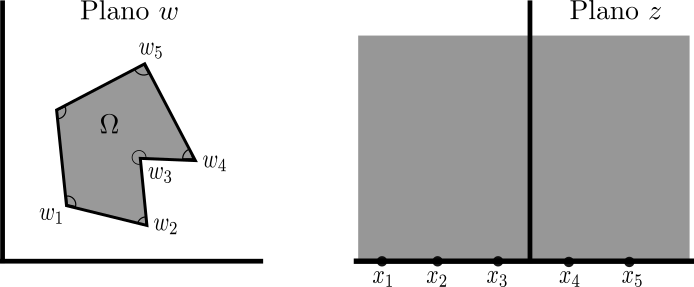
\includegraphics[width=0.7\linewidth]{img/sc}
	\caption{Transformación de Schwarz-Christoffel}
	\label{fig:sc}
\end{figure}
Supongamos que cada $w_j$ se mapea en $x_j$, donde $x_j$ es un punto en el eje real.
La transformación que mapea el semiplano superior en   $\Omega$ está definida  como:

\begin{equation}\label{dSC}
	\dfrac{dw}{dz}=C_1\prod_{j=1}^{n}(z-x_n)^{\frac{\phi_j}{\pi}-1}.
\end{equation}
En forma integral
\begin{equation}\label{eSC}
	w=C_1\int \prod_{j=1}^{n}(z-x_n)^{\frac{\phi_j}{\pi}-1} dz +C_2,
\end{equation}
donde $\phi_1,\ldots,\phi_n$ son los ángulos interiores de los vértices $w_j$.\\
La forma más sencilla de entender porqué funciona la fórmula es considerar una familia de incrementos infinitesimales $dz$ a lo largo del eje real en el plano $Z$, y sus imágenes $dw$ en el plano $W$. La clave es explorar los argumentos (o fases) de estos cambios infinitesimales. Ahora la ecuación. (\ref{dSC}) nos dice que:
\begin{equation}\label{SC1}
	\mbox{Arg}(dw)=\mbox{Arg}(dz)+\mbox{Arg}(C_1)+\sum_{j=1}^{n}\left(\dfrac{\phi_j}{\pi}-1\right)\mbox{Arg}(z-x_j).
\end{equation}

A medida que $z$ se mueve a lo largo del eje real en la dirección positiva, cuando $z$ se encuentra estrictamente entre dos de los $x_j$,  todos los términos (\ref{SC1}) son constantes, lo que implica que $w$ se mueve en línea recta.
Esta es la razón por la cual la imagen en el plano $W$ es poligonal. Ahora, debemos observar qué sucede en las esquinas. Cuando $z$ pasa a través de $x_j$, todos los términos excepto aquellos que involucran a $x_j$, permanecen constantes, pero el factor $\mbox{Arg}(z-x_j)$ toma los siguientes valores:
\[
\mbox{Arg}(z-x_j)=\left\{\begin{array}{ccr}
	\pi, &\mbox{si}&z<x_j\\
	0,&\mbox{si}& z>x_j.
\end{array} \right.
\]
El término 
$$\left(\dfrac{\phi_j}{\pi}-1\right) \mbox{Arg}(z-x_j),$$
salta, por lo tanto, del valor $\phi_j-1$ al valor $0$. La dirección en la que $w$ se está desplazando resulta ser un giro positivo (es decir, en sentido antihorario), por $\pi -\phi_j$. Un cambio de dirección por esta cantidad corresponde a la introducción de una esquina en el polígono con un ángulo interior de $\phi_j$.\\

\iffalse Lo que esta discusión establece es que el eje real se mapea a la frontera de una región poligonal. Esto será suficiente para nuestros propósitos. Se puede ir más allá y establecer que el mapeo es uno a uno y, de hecho, toma el semiplano superior al interior de un polígono. Siempre podemos verificar este último punto calculando valores de muestra de mapeos particulares, como la imagen de $i$. \fi 



\subsection{Algunos comentarios sobre el punto en el infinito y los exponentes}
Podemos asumir que uno de los puntos en el eje real, digamos $x_n$, está en el infinito y que se elimina de la lista de puntos en la transformación. Para ver esto, escribimos, con $x_n <\infty$,

$$C_1=\dfrac{C_1^{'}}{(-x_n)^{\frac{\phi_n}{\pi}-1}},$$
$$\dfrac{\partial w}{\partial z}=C_1^{'}(z-x_1)^{\frac{\phi_1}{\pi}-1}(z-x_2)^{\frac{\phi_2}{\pi}-1}\cdots\left(\dfrac{x_n-z}{x_n}\right)^{\frac{\phi_n}{\pi}-1}.$$

Manteniendo  $C_1^{'}<\infty$ y tomando el límite $x_n\rightarrow \infty$, obtenemos 
$$C_1=\dfrac{C_1^{'}}{(-x_n)^{\frac{\phi_n}{\pi}-1}},$$
$$\dfrac{\partial w}{\partial z}=C_1^{'}(z-x_1)^{\frac{\phi_1}{\pi}-1}(z-x_2)^{\frac{\phi_2}{\pi}-1}\cdots(z-x_{n-1})^{\frac{\phi_{n-1}}{\pi}-1}.$$
Recordemos que la suma de los ángulos exteriores de cualquier polígono cerrado es $2\pi$. Por lo tanto, podemos afirmar que
$$\sum_{k=1}^{n}(\pi-\phi_k)=2\pi,$$
o bien, dividiendo entre $-\pi$
$$\sum_{k=1}^{n}\left(\dfrac{\phi_k}{\pi}-1\right)=-2.$$
Por lo tanto, podemos afirmar que la suma de los exponentes en la fórmula \ref{eSC} es $-2$. Esto es una restricción que resultará útil en la relación entre la fórmula \ref{eSC} para un semiplano y el resultado correspondiente para un disco.

También hay algo de libertad en la elección de los $x_n$. Tenga en cuenta que las constantes $C_1$ y $C_2$ simplemente ajustan el tamaño y la posición del polígono generado por el mapeo. Si establecemos $C_1 = 1 $ y $C_2 = 0$, creamos un polígono, digamos $P'$, que es similar al polígono deseado, digamos $P$, pero no tiene el tamaño correcto y no está en la ubicación correcta. Examinemos la libertad en los $x_j$ dentro de este esquema. Supondremos que $x_n = \infty$ aún no se ha realizado. En estas circunstancias, dado que los ángulos exteriores están fijos, todavía hay restricciones entre los $x_j$. Para que $P'$ sea similar a $P$, dado que los ángulos están fijos, requiere que los lados de $P'$ deban tener longitudes que están en una proporción constante común con los lados correspondientes de $P$. Esto implica $n - 3$ restricciones en los vértices, que a su vez están determinados por las $n$ variables $x_j$.\\
Esto significa que antes de hacer que $x_n = \infty$, tres de los $x_j$ se pueden elegir a voluntad. Si hacemos que $x_n = \infty$, dos de los $x_j$ restantes se pueden elegir. Esta libertad también se puede entender en términos de los requisitos dentro del Teorema de mapeo de Riemann necesarios para hacer que el mapeo sea único: debemos especificar la imagen de un punto complejo  y una dirección para garantizar la unicidad.

\subsection{Deducciones de las fórmulas \\de \SC}
La discusión anterior, aunque es informal nos da una idea de la transformación de \SC. A continuación se esboza una deducción de la fórmula de \SC \; para el semiplano superior
\begin{teor}[Fórmula de \SC \; para el semiplano superior\index{Fórmula de \SC\; para el semiplano superior}]
	Sea $\Omega$ una región simplemente conexa cuya frontera sea un polígono con vértices $w_1,\ldots,w_n$ y ángulos interiores $\phi_1, \ldots,\phi_n $ en sentido antihorario. Sea $f$ cualquier mapeo conforme del semiplano superior $H$ a $\Omega$ con $f (\infty) = w_n$. Entonces
	\begin{equation}\label{SCSP}
		f(z)=C_1\int \prod_{j=1}^{n-1}(z-x_n)^{\frac{\phi_j}{\pi}-1} dz +C_2,
	\end{equation}
	para algunas constantes $C_1$ y $C_2$, donde $w_j=f(x_j)$ para $j=1,2,\ldots,n-1$. \\
	\textbf{Esbozo.}\\Para simplificar, tratamos solo el caso donde todos los $x_j$ son finitos y el producto oscila entre los índices $1$ a $n$. Por el principio de reflexión de Schwarz,  el mapeo $f$ puede continuarse analíticamente en el semiplano inferior; la imagen continúa en el reflejo de $\Omega$ sobre uno de los lados del polígono. Al reflejar de nuevo sobre un lado del nuevo polígono, podemos regresar analíticamente al semiplano superior. Lo mismo se puede hacer para cualquier número par de reflexiones de $\Omega$, cada vez creando una nueva rama de $f$. La imagen de cada rama debe ser una copia trasladada y rotada de $\Omega$. Ahora, si $C_1$ y $C_2$ son constantes complejas, entonces
	$$\dfrac{(C_2+C_1f(z))''}{(C_2+Cf(z))'}=\dfrac{f''(z)}{f'(z)}.$$
	Por lo tanto, la función $\dfrac{f''(z)}{f'(z)}$ se puede definir por  continuación como una función univaluada en todas partes de la cerradura en el semiplano superior, excepto en los $z_j$ (donde las derivadas pueden no existir). Análogamente, considerando números impares de reflexiones, vemos que $\dfrac{f''(z)}{f'(z)}$ 	es univaluada y también es analítica en el semiplano inferior.\\
	Afirmamos que dado $x_j$, se cumple que 
	$$f'(z)=(z-x_j)^{\dfrac{\phi_j}{\pi}-1}\psi(z),$$
	para una función analítica $\psi(z)$ en una vecindad de $x_j$. En efecto, puesto 	que la idea detrás de la transformación \SC \; es que una transformación conforme $f$ pueda tener una derivada que se puede expresar 	como
	$$f'=\prod f_j,$$
	por el principio de reflexión de Schwarz, la función $f$ puede continuarse analíticamente a través del segmento $(x_j,x_{j+1})$.  En particular, $f'$ existe
	en este segmento, y vemos que $\mbox{arg} f'$ debe ser constante allí. Además, $\mbox{arg} f'$ debe experimentar un salto en $z = x_j$, a saber
	$$[\mbox{arg}f'(z)]_{x_j^{-}}^{x_j^{+}}=\left(1-\dfrac{\phi_j}{\pi}\right)\pi=\beta_j\pi.$$
	El ángulo $\beta_j\pi $ es el ángulo de giro en el $j$-ésimo vértice. Ahora identificamos una función $f_j$ que es analítica en el semiplano superior que  satisface $[\mbox{arg}f'(z)]_{x_j^{-}}^{x_j^{+}}=\beta_j\pi $, y  además tiene $\mbox{arg}f_j$ es constante en $\R$:
	$$f_j=(z-x_j)^{-\beta_j},$$
	tomando $f_j(z)>0$ si $z>x_j$ sobre $\R$ podemos formar
	$$f'(z)=K\prod_{j=1}^{n}f_j(z),$$
	donde $K$ es alguna constante. Lo anterior prueba la afirmación.\\
	Ya que $$f'(z)=(z-x_j)^{\frac{\phi_j}{\pi}-1}\psi(z),$$ entonces, $\dfrac{f''(z)}{f'(z)}$  tiene un polo simple en $x_j$ con residuo $\dfrac{\phi_j}{\pi}-1$, y 
	$$\dfrac{f''(z)}{f'(z)}-\ds\sum_{j=1}^{n}\dfrac{\dfrac{\phi_j}{\pi}-1}{z-x_j},$$ es una función entera. Como $x_j<\infty$ para cada $j$, $f$ es analítica en $z=\infty$, y la expansión en series de Laurent implica que  $\dfrac{f''(z)}{f'(z)}\rightarrow0$ cuando $z\rightarrow\infty$, por el Teorema de Liouville se sigue que $$\dfrac{f''(z)}{f'(z)}-\ds\sum_{j=1}^{n}\dfrac{\dfrac{\phi_j}{\pi}-1}{z-x_j},$$
	es idénticamente cero. Expresando $\dfrac{f''}{f}$ como $(\ln (f'))'$ e integrando obtenemos la fórmula de \SC.
\end{teor}
Existe una versión que mapea el disco unitario $D(0,1)$  en un polígono.
\begin{teor}[Fórmula de \SC \; para el disco] \index{Fórmula de \SC \; para el disco}
	Sea $\Omega$ una región simplemente conexa cuya frontera sea un polígono con vértices $w_1,\ldots,w_n$ y ángulos interiores $\phi_1, \ldots,\phi_n $ en sentido antihorario. Sea $f$ cualquier mapeo conforme del disco unitario $D(0,1)$ a $\Omega$. Entonces
	\begin{equation}\label{SCD}
		f(z)=A+C\int\prod_{k=1}^{n}\left(\dfrac{z}{x_k}-1\right)^{\frac{\phi_k}{\pi}-1}dz=\bar{C}\int\prod_{k=1}^{n}(p-p_j)^{\frac{\phi_k}{\pi}-1}dp+\bar{A},
	\end{equation}
	para algunas $A,C\in \C$, donde $w_k=f(x_k)$ para $k=1,2,\ldots,n$.\\
	\textbf{Esbozo.} \\El mapeo 
	$$p(z)=\dfrac{z-i}{z+i},$$
	manda el semiplano superior al circulo unitario. La inversa de este mapeo resulta ser
	$$\dfrac{i(1+p)}{1-p},$$
	suponga que los $x_k$ son mapeados a puntos $p_k$ en el circulo unitario. Entonces, para cada $k$ tenemos
	$$z-x_k=\dfrac{i(p+1)}{1-p}-\dfrac{i(p_k+1)}{1-p_k}=\dfrac{2i(p-p_k)}{(1-p)(1-p_k)},$$
	así como el Jacobiano de la transformación es 
	$$\dfrac{\partial z}{\partial p}=\dfrac{2i}{(1-p)^2},$$
	sustituyendo esto en la fórmula de \SC y usando el exponente de la fórmula 
	$$\sum_{k=1}^{n}\left(\dfrac{\phi_k}{\pi}-1\right)=-2,$$
	y simplificando obtenemos la fórmula.
\end{teor}

%% Continuar aca la revisión

\section{Ejemplos del uso de la fórmula de Schwarz-Christoffel para el semiplano}
En esta sección se presentan una serie de ejemplos que nos permitirán tener una comprensión más clara de la fórmula (\ref{eSC}). Ahora consideraremos algunos ejemplos analíticos simples. No es difícil suponer que  la cuestión se complica un poco más cuando hay más de tres vértices, ya que entonces tenemos que resolver el problema de determinar los $x_j$ para todos excepto tres de los valores de $j$. Así que consideraremos primero algunos casos con solo dos vértices, que se pueden resolver de manera analítica.Así que consideraremos primero algunos casos con solo dos vértices, que se pueden resolver de manera analítica.
\subsection{Polígono con un vértice}
Las fórmulas de \SC \; no son del todo explicitas; debemos determinar los $x_j$ y las constantes afines $C_1$ y $C_2$ antes de poder aplicar la fórmula. Existe cierta flexibilidad en la selección de estos parámetros. Por el Teorema de mapeo de Riemann, podemos elegir cualesquiera tres puntos en $\R\setminus\{\infty\}$ para mapearlos a cualesquiera tres puntos del polígono, siempre y cuando se mantenga su orden. En otras palabras, hay tres grados de libertad en el mapeo, lo que nos permite elegir tres  $x_j$ arbitrariamente. Por lo tanto, si $n \leq 3$, no hay problema de parámetros que debamos resolver y la fórmula \SC \; se vuelve explícita y en ocasiones sencilla de resolver.\\
Cuando $n=1$, el polígono resulta ser una línea, con vértice  $w_1=\infty$ y $\phi_1=-\pi$, entonces $f(z)$ resulta ser de la forma
$$f(z)=C_2+C_1z,$$
que permite el escalado, la rotación y la traslación. La fórmula del mapeo de \SC para el disco, (\ref{SCD}),00 nos da 
$$f(z)=A+\dfrac{C}{z-z_1}.$$
Este es uno de los pocos resultados analíticos simples de la fórmula de Schwarz-Christoffel. 
\subsection{La franja vertical semi-infinita.}
Posiblemente el caso más simple es el de la franja vertical semi-infinita dada por:
$$\Omega=\{ w\in \C : -a\leq \mbox{Re}(w)\leq a\; y \; \mbox{Im}(w)\geq 0  \},$$
donde $a\in\R\setminus{0}$.\\
En este caso tenemos:
\[
\begin{array}{lcr}
	w_1=-a;&&\phi_1=\dfrac{\pi}{2},\\
	w_2=a;&&\phi_2=\dfrac{\pi}{2},
\end{array}
\]
y podemos simplemente tomar $x_1=-1$, $x_2=1$. Entonces la forma diferencial de la ecuación de Schwarz-Chrstoffel nos da
$$\dfrac{\partial w}{\partial z}=C_1(z-1)^{\dfrac{\frac{\pi}{2}}{\pi}-1}(z+1)^{\frac{\frac{\pi}{2}}{\pi}-1}=\dfrac{C_1}{\sqrt{z^2-1}}=\dfrac{A}{\sqrt{1-z^2}},$$
donde el cambio de las constantes lo realizamos para que la ecuación nos sea más fácil de integrar, es decir,
\[
w=\int \dfrac{\partial w}{\partial x}dx=\int \dfrac{A}{\sqrt{1-z^2}}=B+A\sin^{-1}(z).
\]
Ahora las constantes $A$ y $B$ se pueden fijar mirando las ubicaciones de los vértices. Considerando el primer vértice, esto nos da:
$$-a=B+A\sin^{-1}(-1)=B-\dfrac{A\pi}{2}.$$
El otro vértice nos da
$$a=B+A\sin^{-1}(1)=B+\dfrac{A\pi}{2},$$
resolviendo el sistema $2\times2$ que se obtuvo, se tiene que $B=0$ y por consiguiente $$A=\dfrac{2a}{\pi},$$
así pues 
\[
\begin{array}{lcr}
	w=\dfrac{2a\sin^{-1}(z)}{\pi},&&z=\sin\left(\dfrac{\pi w}{2a}\right),
\end{array}
\]
Consideremos cuando $a=1$, es decir
\[
\begin{array}{lcr}
	w=\dfrac{2\sin^{-1}(z)}{\pi},&&z=\sin\left(\dfrac{\pi w}{2}\right),
\end{array}
\]
Podemos tener una mirada más detallada a lo que hace este mapeo usando las funciones que se construyeron en el capítulo 2.

\begin{mmaCell}{Input}
	 cartesianMap[func_, xrange_, yrange_, options___] := \\ParametricPlot[Evaluate[Through[\{Re, Im\}[func]]],\\xrange, yrange, options]
\end{mmaCell}

\begin{mmaCell}{Input}
	 cartesianConformal[func_, xrange_, yrange_, options___] :=\\Show[GraphicsGrid[\{\{cartesianMap[x + I*y, xrange, yrange,\\options,DisplayFunction -> Identity],\\cartesianMap[W[x + I*y],xrange, yrange, options,\\DisplayFunction -> Identity]\}\}],\\DisplayFunction -> \$DisplayFunction]
\end{mmaCell}


\begin{mmaCell}{Input}
	  w[z_] = (2*ArcSin[z])/Pi;\\cartesianConformal[w[x + I*y], \{x, -16, 16\}, \{y, 10^(-8), 16\},\\Mesh -> 50, LabelStyle -> Directive[Larger, Bold],\\PlotStyle -> White, MeshStyle -> Blue, Axes -> True,\\PlotPoints -> 200, PlotRange -> All]
\end{mmaCell}
\begin{mmaCell}[moregraphics={moreig={scale=0.4}}]{Output}
	\mmaFrac{ \mmaGraphics{28.png}}{}
\end{mmaCell}

\subsection{Triángulos}


Los polígonos con tres vértices son los dominios más generales para los cuales los $x_j$ de la fórmula de Schwarz-Christoffel pueden elegirse arbitrariamente, siempre y cuando permanezcan distintos y estén ordenados correctamente. Consideremos la siguiente imagen (los parámetros en la rutina de trazado son con fines ilustrativos y no tienen un significado en particular), donde asumimos que el punto $A$ está en el origen y $B$ está en $w = 1 + 0i = 1$. Los ángulos interiores en estos dos vértices son $\alpha$ y $\beta$, respectivamente.

\begin{mmaCell}{Input}
	 Show[Graphics[\{\{LightBlue,Polygon[\{\{0,0\},\{1,0\},\{0.3,1\}\}]\},\\ \{PointSize[0.03], Point[\{0, 0\}]\},\{PointSize[0.03],\\Point[\{1, 0\}]\},\{PointSize[0.03], Point[\{0.3, 1\}]\}, \\Line[\{\{-1/2, 0\}, \{1.5, 0\}\}],Line[\{\{0, -1/2\}, \{0, 1.5\}\}],\\Text["A", \{0.1, -0.1\}], Text["B", \{1.1, -0.1\}],\\Text["C", \{0.3, 1.2\}],Text["[Alpha]", \{0.1, 0.1\}],\\Text["[Beta]", \{0.85, 0.1\}]\}]]
\end{mmaCell}

\begin{mmaCell}[moregraphics={moreig={scale=0.4}}]{Output}
	\mmaFrac{ \mmaGraphics{29.png}}{}
\end{mmaCell}

Lo que buscamos es construir de alguna manera un mapeo $w(z)$ tal que este triángulo sea la imagen del plano superior, con A situado en el origen z = 0, y B en z = 1. Aquí haremos uso del hecho de que $C$ puede ser definido como $f(\infty)=C$, de modo que la fórmula \SC \; solo involucre dos términos:
$$\dfrac{\partial w}{\partial z}=A' z^{\frac{\alpha}{\pi}-1}(z-1)^{\frac{\beta}{\pi}-1}=Cz^{\frac{\alpha}{\pi}-1}(1-z)^{\frac{\beta}{\pi}-1},$$
integrando desde $\xi=0$ hasta $\xi=z$
$$w=C\int_{0}^{z}\xi^{\frac{\alpha}{\pi}-1}(1-\xi)^{\frac{\beta}{\pi}-1}d\xi+B.$$
Ahora, cuando $z = 0$, también queremos que $w = 0$, por lo que ponemos $B = 0$. Además, dado que $w = 1$ cuando $z = 1$, debemos elegir a $C$ tal que se cumpla:
$$1=C\int_{0}^{1}\xi^{\frac{\alpha}{\pi}-1}(1-\xi)^{\frac{\beta}{\pi}-1}d\xi+B.$$
Utilizamos a continuación la función \textbf{Integrate} de Mathematica
\begin{mmaCell}{Input}
	 Integrate[\mmaSup{\mmaFnc{\(\pmb{\xi}\)}}{\mmaFrac{\mmaUnd{\(\pmb{\alpha}\)}}{\mmaDef{\(\pmb{\pi}\)}}-1}\mmaSup{(1-\mmaFnc{\(\pmb{\xi}\)})}{\mmaFrac{\mmaUnd{\(\pmb{\beta}\)}}{\mmaDef{\(\pmb{\pi}\)}}-1},\{\mmaFnc{\(\pmb{\xi}\)},0,1\},Assumptions\(\pmb{\to}\)\{\mmaUnd{\(\pmb{\alpha}\)}>0,\mmaUnd{\(\pmb{\beta}\)}>0\}]
\end{mmaCell}
obtenemos
$$\dfrac{\Gamma\left(\dfrac{\alpha}{\pi}\right)\Gamma\left(\dfrac{\beta}{\pi}\right)}{\Gamma\left(\dfrac{\alpha+\beta}{\pi}\right)},$$
por lo tanto 
$$C=\dfrac{\Gamma\left(\dfrac{\alpha+\beta}{\pi}\right)}{\Gamma\left(\dfrac{\alpha}{\pi}\right)\Gamma\left(\dfrac{\beta}{\pi}\right)},$$
por consiguiente, el mapeo viene dado por 
\begin{equation}
	w=\dfrac{\Gamma\left(\dfrac{\alpha+\beta}{\pi}\right)}{\Gamma\left(\dfrac{\alpha}{\pi}\right)\Gamma\left(\dfrac{\beta}{\pi}\right)}\int_{0}^{z}\xi^{\frac{\alpha}{\pi}-1}(1-\xi)^{\frac{\beta}{\pi}-1}d\xi.
\end{equation}
Recordemos que  $$\int_{0}^{z}\xi^{a-1}(1-\xi)^{b-1}d\xi = \beta_z(a,b),$$
donde $\beta_z(a,b)$ es la función beta incompleta. En \textbf{Mathematica}, esta función especial puede usarse utilizando el comando \textbf{Beta[z,a,b]}.\\
Por otro lado, la función Beta se puede expresar en términos de la función Gamma
\[
{\displaystyle {\begin{aligned}\Gamma (x)\Gamma (y)&=\int _{u=0}^{\infty }u^{x-1}e^{-u}du\int _{v=0}^{\infty }v^{y-1}e^{-v}dv\\&=\int _{v=0}^{\infty }\int _{u=0}^{\infty }u^{x-1}v^{y-1}e^{-u-v}dudv,\end{aligned}}}
\]
haciendo el cambio $u=zt$ y $v=z(1-t)$

\[
\displaystyle {\begin{aligned}\Gamma (x)\Gamma (y)&=\int _{z=0}^{\infty }\int _{t=0}^{1}e^{-z}(zt)^{x-1}(z(1-t))^{y-1}zdtdz\\&=\int _{z=0}^{\infty }e^{-z}z^{x+y-1}dz\int _{t=0}^{1}t^{x-1}(1-t)^{y-1}dt\\&=\Gamma (x+y)\beta (x,y),\end{aligned}}
\]
despejando obtenemos
\[
{\displaystyle \beta (x,y)={\dfrac {\Gamma (x)\Gamma (y)}{\Gamma (x+y)}}}.
\]
En \textbf{Mathematica}, la función beta se puede usar usando el comando \textbf{Beta[a,b]}. Así, 
$$w=\dfrac{\beta_z\left(\dfrac{\alpha}{\pi},\dfrac{\beta}{\pi}\right)}{\beta\left(\dfrac{\alpha}{\pi},\dfrac{\beta}{\pi}\right)},$$
teniendo esto en cuenta, escribimos la expresión para $w$ en \textbf{Mathematica}
\begin{mmaCell}{Input}
	 w[z_,\(\alpha\)_,\(\beta\)_]:=\mmaFrac{Beta[z,\(\alpha\),\(\beta\)]}{Beta[\(\alpha\),\(\beta\)]}
\end{mmaCell}
En \textbf{Mathematica}, contamos con una función que simplifica a la expresión anterior. Esta es la función \textbf{BetaRegularized}, esta función da la función beta incompleta regularizada $I_z(a,b)$. Para casos no singulares, se verifica que
$$I_z(a,b)=\dfrac{\beta(z,a,b)}{\beta(a,b)}.$$
Ya con esto podemos reescribir a $w$ en Wolfram de la siguiente manera
\begin{mmaCell}{Input}
	 w[z_,\(\alpha\)_,\(\beta\)_]:=BetaRegularized[z,\(\alpha\),\(\beta\)]
\end{mmaCell}
Verifiquemos esta fórmula para el caso en el que el triángulo es equilátero, con $\alpha=\beta=\dfrac{\pi}{3}$
\begin{mmaCell}{Input}
	 ClearAll[z, w, k]\\w[z_] = BetaRegularized[z, 1/3, 1/3]\\cartesianConformal[w[x + I*y],\{x, -8, 8\}, \{y, 10^(-12), 8\},\\Mesh -> 60, LabelStyle -> Directive[Larger, Bold],\\PlotStyle -> AbsoluteThickness[0.01], MeshStyle -> Blue,\\Axes -> True,PlotPoints -> 1000, PlotRange -> All]
\end{mmaCell}
\begin{mmaCell}[moregraphics={moreig={scale=0.4}}]{Output}
	\mmaFrac{ \mmaGraphics{30.png}}{}
\end{mmaCell}
\subsection{Rectángulos y funciones elípticas}
Si $n = 4$, los $x_j$ de la fórmula de \SC\;  no pueden ser seleccionados a nuestra elección. En el caso general, no existe una manera analítica con respecto al grado de libertad en los $x_j$. Sin embargo, en el caso importante cuando la región es el interior de un rectángulo, podemos utilizar la simetría para encontrar una solución explícita.\\
\begin{figure}[h!]
	\centering
	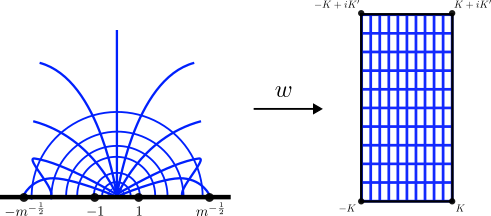
\includegraphics[width=0.72\linewidth]{img/SCR}
	\caption{Mapeo del semiplano superior a un rectángulo}
	\label{fig:scr}
\end{figure}
Rotamos y trasladamos el rectángulo para que sus vértices sean $w_1=-K+iK$, $w_2=-K$, $w_3=K$ y $w_4=K+iK$. Por simetría, elegimos los $x_j$ como $z_1 = -m$, $z_2 = -1$, $z_3 = 1$ y $z_4 = m$,  donde $m$ es un parámetro que representa el grado de libertad en los $x_j$. La imagen del infinito resulta ser  el punto $iK'$, y la imagen de $0$ es $0$. La función puede escribirse como una integral elíptica de primera clase:
\[
\begin{array}{ccl}
	w&=&C_1\ds\int_{}^{z}\prod_{j=1}^{4}(t-x_j)^{-\frac{1}{2}}dt+C_2\\
	&=&-C_1\ds\int_{}^{z}\dfrac{dt}{\sqrt{(m^{2}-t^2)(1-t^2)}},
\end{array}
\]
resulta más conveniente hacer el cambio de variable $a=m^{-1}$, $C_1'=-C_1$, entonces 
\[
\begin{array}{ccl}
	w&=&C_1'\ds\int_{}^{z}\dfrac{dt}{\sqrt{(1-a^2t^2)(1-t^2)}}\\
	=&=&C_1'\ds\int_{}^{\sin^{-1}(z)}\dfrac{d\theta}{\sqrt{1-a^2\sin^2(\theta)}},
\end{array}
\]
Esta integral se conoce como integral elíptica incompleta de primera clase. \textbf{Mathematica} cuenta con una serie de funciones ya definidas para las integrales elípticas. En este ejemplo, la función que usaremos sería  \textbf{EllipticF[$\phi$, m]} la cual nos da la integral elíptica de primer orden $F(\phi|m)$.\\
Ingresando esta última integral en \textbf{Mathematica}
\begin{mmaCell}{Input}
	 Integrate[1/(Sqrt[1 - a*Sin[z]^2]), \{z, 0, ArcSin[z]\}]
\end{mmaCell}
obtenemos el siguiente resultado\\
\fbox{$F\left(\left.\sin ^{-1}(z)\right|a\right)\text{ if }0<\R\left(\sin ^{-1}(z)\right)\leq \dfrac{\pi }{2}\lor -\dfrac{\pi }{2}\leq \R\left(\sin ^{-1}(z)\right)<0$}\\
Para obtener información más detallada sobre estas funciones en \textbf{Mathematica}, consulte \cite{Elliptic}.\\
Para simplificar,  tomemos $c_1'=1$ y $m=2$, entonces $a=\dfrac{1}{2}$.
\begin{mmaCell}{Input}
	 ClearAll[z, w];\\w[z_] = EllipticF[ArcSin[z], 0.5^2];\\cartesianConformal[w[x + I*y], {x, -8, 8}, \{y, 10^(-12), 8\},\\Mesh -> 60, LabelStyle -> Directive[Larger, Bold],\\PlotStyle -> AbsoluteThickness[0.01], MeshStyle -> Blue,\\Axes -> True, PlotPoints -> 1000, PlotRange -> All]
\end{mmaCell}
\begin{mmaCell}[moregraphics={moreig={scale=0.4}}]{Output}
	\mmaFrac{ \mmaGraphics{31.png}}{}
\end{mmaCell}
\section{Ejemplos del uso de la fórmula de Schwarz-Christoffel para el disco unitario}
En este caso, podemos hacer uso de la simetría para considerar puntos $p_j$ que estén espaciados uniformemente alrededor del círculo unitario, Incluso podemos tomar los puntos $_j$ de tal forma que sean las raíces $n$-ésimas de la unidad, es decir, 
$$p_j=\omega_n^j,$$
$$\omega_n^{\frac{2\pi i}{n}}.$$
El producto $(p-p_1)\cdots (p-p_n)$ se simplifica a $p^n-1$. Si nuestro objetivo es un $n$-ágono regular, los ángulos interiores para un $n$-ágono son todos iguales y están dados por:
$$\phi_k=\pi\left(1-\dfrac{2}{n}\right),$$
y los exponentes son todos iguales a $-\dfrac{2}{n}$. Por lo tanto, el mapeo deseado es de la forma 
\begin{equation}
	w=\bar{A}\ds\int \dfrac{dp}{(p^n-1)^{\frac{n}{2}}}+B.
\end{equation} 
Considerando los límites desde $p=0$ hasta $p=z$ y tomando $A=1$ obtendremos resultados más claros
\begin{equation}\label{SCn}
	w=\ds\int_{0}^{z}\dfrac{dp}{(1-p^n)^{\frac{n}{2}}}.
\end{equation}
\subsection{El hexágono}
Se obtiene un hexágono regular al establecer $n = 6$ en la ecuación (\ref{SCn}).
\begin{mmaCell}{Input}
  	 Integrate[1/(1 - p^6)^(1/3), {p, 0, z}]
\end{mmaCell} 
\vspace{-0.5 cm}donde obtenemos\\
\fbox{$z \, _2F_1\left(\dfrac{1}{6},\dfrac{1}{3};\dfrac{7}{6};z^6\right)\text{ if }-1<\text{Re} z\leq 1\lor z\notin \mathbb{R}$}\\
donde $_2F_1$ es la función hipergeométrica, en \textbf{Mathematica} esta función se escribe \textbf{ Hypergeometric2F1[a,b,c,z] }. Para más detalles puede consultar \cite{Hypergeometric2F1}.\\
Para comprobar qué está haciendo esta función usamos la función \textbf{polarConformal} que construimos anteriormente
\begin{mmaCell}{Input}
	 ClearAll[f, z]\\f[z_] = z Hypergeometric2F1[1/6, 1/3, 7/6, z^6]\\polarConformal[f[r Exp[I*t]], {r, 0, 1},\\\{t, 0, 2*Pi\},Mesh -> \{50, 50\}, PlotRange -> All,\\LabelStyle -> Directive[Larger, Bold], PlotStyle -> White,\\MeshStyle -> Blue, Axes -> True]
\end{mmaCell}
\begin{mmaCell}[moregraphics={moreig={scale=0.4}}]{Output}
	\mmaFrac{ \mmaGraphics{32.png}}{}
\end{mmaCell}

\subsection{El $n$-ágono regular}
Con las consideraciones hechas previamente, ahora nos resulta sencillo tratar el $n$-ágono regular
\begin{mmaCell}{Input}
	 nAgon[z_, n_] = Integrate[1/(1 - p^n)^(2/n), \{p, 0, z\},\\Assumptions -> n > 0]]
\end{mmaCell} 
obtenemos la siguiente expresión en términos de la función hipergeométrica
$$z \, _2F_1\left(\dfrac{1}{n},\dfrac{2}{n};1+\dfrac{1}{n};z^n\right).$$
Ahora, solo basta cambiar el parámetro $n$.\\
Las siguientes imágenes se generaron usando $n=3,4,5,10$ en el código
\begin{mmaCell}{Input}
	 ClearAll[f, z]\\polarConformal[nAgon[r Exp[I*t], n], \{r, 0, 1\},\{t, 0, 2*Pi\},\\Mesh -> \{100, 100\}, PlotRange -> All,\\LabelStyle -> Directive[Larger, Bold],PlotStyle -> White,\\MeshStyle -> Blue, Axes -> True]
\end{mmaCell}
las imágenes obtenidas las podemos ver en la figura \ref{fig:Mapeo del círculo unitario al n-ágono}. 
\begin{figure}[htbp]
	\centering
	\begin{subfigure}{0.45\textwidth}
		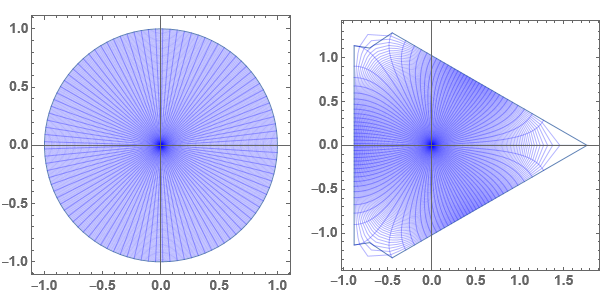
\includegraphics[width=\linewidth]{33.png}
		\caption{Mapeo del círculo unitario al triángulo.}
		\label{fig:Mapeo del círculo unitario al triángulo.}
	\end{subfigure}
	\begin{subfigure}{0.45\textwidth}
		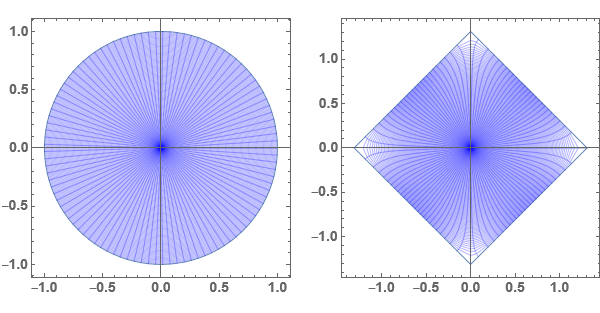
\includegraphics[width=\linewidth]{34.png}
		\caption{Mapeo del círculo unitario al cuadrado.}
		\label{fig:Mapeo del círculo unitario al cuadrado}
	\end{subfigure}
	
	\begin{subfigure}{0.45\textwidth}
		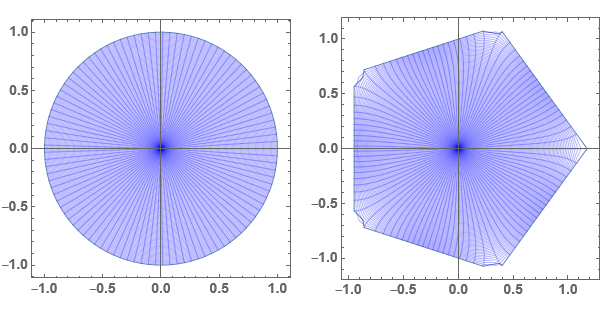
\includegraphics[width=\linewidth]{35.png}
		\caption{Mapeo del círculo unitario al pentágono.}
		\label{fig:Mapeo del círculo unitario al pentágono}
	\end{subfigure}
	\begin{subfigure}{0.45\textwidth}
		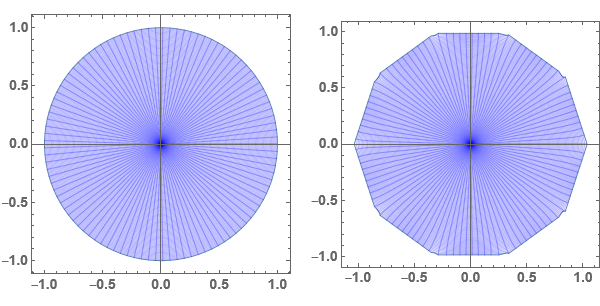
\includegraphics[width=\linewidth]{36.png}
		\caption{Mapeo del círculo unitario al decágono.}
		\label{fig:Mapeo del círculo unitario al decágono}
	\end{subfigure}
	\caption{Mapeo del círculo unitario al n-ágono}
	\label{fig:Mapeo del círculo unitario al n-ágono}
\end{figure}




